% Options for packages loaded elsewhere
\PassOptionsToPackage{unicode}{hyperref}
\PassOptionsToPackage{hyphens}{url}
\PassOptionsToPackage{dvipsnames,svgnames,x11names}{xcolor}
%
\documentclass[
  10pt,
  dvipsnames,enabledeprecatedfontcommands]{scrartcl}
\usepackage{amsmath,amssymb}
\usepackage{lmodern}
\usepackage{iftex}
\ifPDFTeX
  \usepackage[T1]{fontenc}
  \usepackage[utf8]{inputenc}
  \usepackage{textcomp} % provide euro and other symbols
\else % if luatex or xetex
  \usepackage{unicode-math}
  \defaultfontfeatures{Scale=MatchLowercase}
  \defaultfontfeatures[\rmfamily]{Ligatures=TeX,Scale=1}
\fi
% Use upquote if available, for straight quotes in verbatim environments
\IfFileExists{upquote.sty}{\usepackage{upquote}}{}
\IfFileExists{microtype.sty}{% use microtype if available
  \usepackage[]{microtype}
  \UseMicrotypeSet[protrusion]{basicmath} % disable protrusion for tt fonts
}{}
\usepackage{xcolor}
\usepackage{graphicx}
\makeatletter
\def\maxwidth{\ifdim\Gin@nat@width>\linewidth\linewidth\else\Gin@nat@width\fi}
\def\maxheight{\ifdim\Gin@nat@height>\textheight\textheight\else\Gin@nat@height\fi}
\makeatother
% Scale images if necessary, so that they will not overflow the page
% margins by default, and it is still possible to overwrite the defaults
% using explicit options in \includegraphics[width, height, ...]{}
\setkeys{Gin}{width=\maxwidth,height=\maxheight,keepaspectratio}
% Set default figure placement to htbp
\makeatletter
\def\fps@figure{htbp}
\makeatother
\setlength{\emergencystretch}{3em} % prevent overfull lines
\providecommand{\tightlist}{%
  \setlength{\itemsep}{0pt}\setlength{\parskip}{0pt}}
\setcounter{secnumdepth}{5}
\newlength{\cslhangindent}
\setlength{\cslhangindent}{1.5em}
\newlength{\csllabelwidth}
\setlength{\csllabelwidth}{3em}
\newlength{\cslentryspacingunit} % times entry-spacing
\setlength{\cslentryspacingunit}{\parskip}
\newenvironment{CSLReferences}[2] % #1 hanging-ident, #2 entry spacing
 {% don't indent paragraphs
  \setlength{\parindent}{0pt}
  % turn on hanging indent if param 1 is 1
  \ifodd #1
  \let\oldpar\par
  \def\par{\hangindent=\cslhangindent\oldpar}
  \fi
  % set entry spacing
  \setlength{\parskip}{#2\cslentryspacingunit}
 }%
 {}
\usepackage{calc}
\newcommand{\CSLBlock}[1]{#1\hfill\break}
\newcommand{\CSLLeftMargin}[1]{\parbox[t]{\csllabelwidth}{#1}}
\newcommand{\CSLRightInline}[1]{\parbox[t]{\linewidth - \csllabelwidth}{#1}\break}
\newcommand{\CSLIndent}[1]{\hspace{\cslhangindent}#1}
%\documentclass{article}

% %packages
 \usepackage{booktabs}
\usepackage{subcaption}
\usepackage{multirow}
\usepackage{colortbl}
\usepackage{graphicx}
\usepackage{longtable}
\usepackage{ragged2e}
\usepackage{etex}
%\usepackage{yfonts}
\usepackage{marvosym}
\usepackage[notextcomp]{kpfonts}
\usepackage{nicefrac}
\newcommand*{\QED}{\hfill \footnotesize {\sc Q.e.d.}}
\usepackage{floatrow}
%\usepackage[titletoc]{appendix}
%\renewcommand\thesubsection{\Alph{subsection}}

\usepackage[textsize=footnotesize]{todonotes}
\newcommand{\ali}[1]{\todo[color=gray!40]{#1}}
\newcommand{\mar}[1]{\todo[color=blue!40]{#1}}
\newcommand{\raf}[1]{\todo[color=olive!40]{#1}}
%\linespread{1.5}
\newcommand{\indep}{\!\perp \!\!\! \perp\!}


\setlength{\parindent}{10pt}
\setlength{\parskip}{1pt}


%language
\usepackage{times}
\usepackage{t1enc}
%\usepackage[utf8x]{inputenc}
%\usepackage[polish]{babel}
%\usepackage{polski}




%AMS
\usepackage{amsfonts}
\usepackage{amssymb}
\usepackage{amsthm}
\usepackage{amsmath}
\usepackage{mathtools}

\usepackage{geometry}
 \geometry{a4paper,left=35mm,top=20mm,}


%environments
\newtheorem{fact}{Fact}



%abbreviations
\newcommand{\ra}{\rangle}
\newcommand{\la}{\langle}
\newcommand{\n}{\neg}
\newcommand{\et}{\wedge}
\newcommand{\jt}{\rightarrow}
\newcommand{\ko}[1]{\forall  #1\,}
\newcommand{\ro}{\leftrightarrow}
\newcommand{\exi}[1]{\exists\, {_{#1}}}
\newcommand{\pr}[1]{\mathsf{P}(#1)}
\newcommand{\cost}{\mathsf{cost}}
\newcommand{\benefit}{\mathsf{benefit}}
\newcommand{\ut}{\mathsf{ut}}

\newcommand{\odds}{\mathsf{Odds}}
\newcommand{\ind}{\mathsf{Ind}}
\newcommand{\nf}[2]{\nicefrac{#1\,}{#2}}
\newcommand{\R}[1]{\texttt{#1}}
\newcommand{\prr}[1]{\mbox{$\mathtt{P}_{prior}(#1)$}}
\newcommand{\prp}[1]{\mbox{$\mathtt{P}_{posterior}(#1)$}}



\newtheorem{q}{\color{blue}Question}
\newtheorem{lemma}{Lemma}
\newtheorem{theorem}{Theorem}



%technical intermezzo
%---------------------

\newcommand{\intermezzoa}{
	\begin{minipage}[c]{13cm}
	\begin{center}\rule{10cm}{0.4pt}



	\tiny{\sc Optional Content Starts}
	
	\vspace{-1mm}
	
	\rule{10cm}{0.4pt}\end{center}
	\end{minipage}\nopagebreak 
	}


\newcommand{\intermezzob}{\nopagebreak 
	\begin{minipage}[c]{13cm}
	\begin{center}\rule{10cm}{0.4pt}

	\tiny{\sc Optional Content Ends}
	
	\vspace{-1mm}
	
	\rule{10cm}{0.4pt}\end{center}
	\end{minipage}
	}
%--------------------






















\newtheorem*{reply*}{Reply}
\usepackage{enumitem}
\newcommand{\question}[1]{\begin{enumerate}[resume,leftmargin=0cm,labelsep=0cm,align=left]
\item #1
\end{enumerate}}

\usepackage{float}

% \setbeamertemplate{blocks}[rounded][shadow=true]
% \setbeamertemplate{itemize items}[ball]
% \AtBeginPart{}
% \AtBeginSection{}
% \AtBeginSubsection{}
% \AtBeginSubsubsection{}
% \setlength{\emergencystretch}{0em}
% \setlength{\parskip}{0pt}






\usepackage[authoryear]{natbib}

%\bibliographystyle{apalike}



\usepackage{tikz}
\usetikzlibrary{positioning,shapes,arrows}

\ifLuaTeX
  \usepackage{selnolig}  % disable illegal ligatures
\fi
\IfFileExists{bookmark.sty}{\usepackage{bookmark}}{\usepackage{hyperref}}
\IfFileExists{xurl.sty}{\usepackage{xurl}}{} % add URL line breaks if available
\urlstyle{same} % disable monospaced font for URLs
\hypersetup{
  pdftitle={``Weight of Evidence, Evidential Completeness and Accuracy''},
  pdfauthor={Rafal Urbaniak and Marcello Di Bello},
  colorlinks=true,
  linkcolor={Maroon},
  filecolor={Maroon},
  citecolor={Blue},
  urlcolor={blue},
  pdfcreator={LaTeX via pandoc}}

\title{``Weight of Evidence, Evidential Completeness and Accuracy''}
\author{Rafal Urbaniak and Marcello Di Bello}
\date{}

\begin{document}
\maketitle

\hypertarget{balance-vs.-weight}{%
\section{Balance vs.~weight}\label{balance-vs.-weight}}

Suppose we want to represent our uncertainty about a proposition in
terms of a single probability that we assign to it. It is not too
difficult to inspire the intuition that this representation does not
capture an important dimension of how our uncertainty connects with the
evidence we have or have not obtained. In a 1872 manuscript of
\emph{The Fixation of Belief} (W3 295) C. S. Peirce gives an example
meant to do exactly that.

\begin{quote} When we have drawn a thousand times, if about half have been white, we have great confidence in this result. We now feel pretty sure that, if we were to make a large number of bets upon the color of single beans drawn from the bag, we could approximately insure ourselves in the long run by betting each time upon the white, a confidence which would be entirely wanting if, instead of sampling the bag by 1000 drawings, we had done so by only two.
\end{quote}

\noindent The objection is not too complicated. Your best estimate of
the probability of \(W=\)`the next bean will be white' is .5 if half of
the beans you have drawn randomly so far have been white, no matter
whether you have drawn a thousand or only two of them. But this means
that expressing your uncertainty about \(W\) by locutions such as ``my
confidence in \(W\) is .5' does not capture this intuitively important
distinction.

Similar remarks can be found in Peirce's 1878
\emph{Probability of Induction}. There, he also proposes to represent
uncertainty by at least two numbers, the first depending on the inferred
probability, and the second measuring the amount of knowledge obtained;
as the latter, Peirce proposed to use some dispersion-related measure of
error (but then suggested that an error of that estimate should also be
estimated and so, so that ideally more numbers representing errors would
be needed).

Peirce himself did not call this the weight of evidence (and in fact,
used the phrase rather to refer to the balance of evidence, W3 294)
{[}CITE KASSER 2015{]}. However, his criticism of such an oversimplified
representation of uncertainty anticipated what came to be called weight
of evidence by Keynes in his 1921 \emph{A Treatise on Probability}:

\begin{quote}
As the relevant evidence at our disposal increases, the magnitude of the
probability of the argument may either increase or decrease, according as the new knowledge strengthens the unfavourable or the favourable evidence; but something seems to have increased in either case,—we have a more substantial basis upon which to rest our conclusion. I express this by saying that an accession of new evidence increases the weight of an argument. New evidence will sometimes decrease the probability of an argument but it will always increase its `weight.' (p. 71)
\end{quote}

\noindent The key point is the same {[}CITE LEVI 2001{]}: the balance of
probability alone cannot characterize all important aspects of
evidential appraisal. Keynes also considered measuring weight of
evidence in terms of the variance of the posterior distribution of a
certain parameter, but was quite attached to the idea that weight should
increase with new information, even if the dispersion increase with new
evidence {[}TP 80-82{]}, and so he proposed only a very rough sketch of
a positive sketch. Moreover, as he was uncertain how a measure of weight
should be incorporated in further decision-making, the was skeptical
about the practical significance of the notion. {[}TP 83{]}

But what is this positive sketch? On one hand, Keynes {[}TP 58-59{]}
connects the notion of weight with relevance. Call evidence \(E\)
relevant to \(X\) given \(K\) just in case
\(\mathsf{Pr}(X\vert K \wedge E) \neq \mathsf{Pr}(X \vert K)\).\footnote{
  Keynes also uses a slightly more convoluted notion of relevance to
  avoid equally strong items of opposite evidence turning out to be
  irrelevant (this objection has also been brought up by {[}COHEN 1986
  TWELVE{]}). The more complex version is that a proposition \(E_1\) is
  relevant to \(X\) given \(K\) just in case it entails a proposition
  \(E_2\) such that
  \(\pr{X\vert K \wedge E_2} \neq \mathsf{Pr}(X \vert K)\). {[}COHEN
  1986 TWELVE{]} complaints that this still runs into difficulties.
  Ignore \(K\), take an irrelevant proposition \(Z\). It entails
  \(Z\vee X\) and \(\pr{Z \vee X\vert X \wedge E}=1\). Now, by Bayes'
  theorem we have
  \(\pr{X \vert E \wedge (Z \vee X)} = \frac{\pr{X \vert E}\times \pr{Z \vee X \vert X \wedge E}}{\pr{Z \vee X \vert E}} = \frac{\pr{X \vert E}}{\pr{Z \vee X \vert E}}\).
  If the denominator differs from 1, the result differs from the
  numerator. We will ignore such difficulties, as they are not of key
  importance for the development of this chapter.} One postulate than
can be found in the \emph{Treatise} {[}TP 84{]} is:\footnote{RUNDE 1990
  283 suggests Keynes allows for weight of evidence to decrease when new
  evidence increases the range of alternatives, but this is based on
  Keynes' claim that weight is increased when the number of alternatives
  is reduced, and Keynes does not directly say anything about the
  possibility of an increase of the number of alternatives.}

\begin{tabular}{lp{11cm}}
(Monotonicity) & If $E$ is relevant to $X$ given $K$, where $K$ is background knowledge, $V(X\vert K \wedge E) > V(X\vert K)$, where $V$ is the weight of evidence.
\end{tabular}

{[}RUNDE 1990, 280{]} suggests that Keynes at some point calls weight
the completeness of information. This however, is a bit hasty, as Keynes
only says that
\emph{the degree of completeness of the information on which a probability is based does seem to be relevant, as well as the actual magnitude of the probabiltiy, in making practical decisions}.
As later on we will argue that it is actually useful to distinguish
evidential weight (how much evidence do we have?) and evidential
completeness (do we have all the evidence that we would expect in a
given case?), we rather prefer to extract a more modest postulate:

\begin{tabular}{lp{11cm}}
(Completeness) & If $E_1$ and $E_2$ are relevant items of evidence, and $E_2$ is (in a sense to be discussed) more complete than $E_1$,  $V(X\vert K \wedge E_2) > V(X\vert K \wedge E_1)$.
\end{tabular}

\noindent If we conceptualize \(E_2\) being complete and \(E_1\) being
incomplete as \(E_2\) being a maximal relevant conjunction of relevant
claims one of which is \(E_1\), (Completeness) follows from
(Monotonicity).

Similar requirements seem to be inspired by the urn example. We put them
in two forms, a weaker and a stronger one.

\begin{tabular}{lp{11cm}}
  (Weak increase) & In cases analogous to the urn example, the weight obtained by a larger sample is higher, if the frequencies in the samples remain the same.\\
  (Strong increase) & In cases analogous to the urn example, the weight obtained by a larger sample is higher.
  \end{tabular}

Now, some requirements on how weight of evidence is related to the
balance of probability. For one thing, Keynes insists that new
(relevant) evidence might decrease probability but will always increase
weight {[}TP 77{]}. Since (Monotonicity) already captures the idea that
weight will always increase, here we extract the other part of the
claim:

\begin{tabular}{lp{11cm}}
(Possible decrease) & It is possible that   $V(X\vert K \wedge E) > V(X\vert K)$ while $\pr{X \vert K \wedge E} <  \pr {X\vert K}$.
\end{tabular}

Clearly, Keynes also endorsed the following two requirements of a very
similar form:

\begin{tabular}{lp{11cm}}
(Possible increase) & It is possible that   $V(X\vert K \wedge E) > V(X\vert K)$ while $\pr{X \vert K \wedge E} >  \pr {X\vert K}$. \\
(Possibly no change ) & It is possible that   $V(X\vert K \wedge E) > V(X\vert K)$ while $\pr{X \vert K \wedge E} =  \pr {X\vert K}$.
\end{tabular}

Now, back to the urn example. You might think the actually frequency
observed should contribute more to the balance, not to the weight, at
least in the sense that with the same number of observations, more
extreme frequencies should not have lower weight:

\begin{tabular}{lp{11cm}}
(Frequency monotonicity) & For a fixed number of observations in a binomial experiment, for two observed frequencies $f_1$ and $f_2$, if $f_2$ is closer to $.5$ than $f_1$, the weight of observing $f_1$ is not less than that of observing $f_2$.
\end{tabular}

Interestingly, Keynes for quite a few years did not attempt to provide
anything close to a formal explication of the notion, and did not spend
too much time studying the issue. Various reasons for this has been
proposed the literature, a prominent one {[}CITE FEDUZI 2010{]} being
that from the decision-theoretic perspective no clear stopping rule
emerged as to whether the evidence is weighty enough to make a decision.
\todo{Should I talk about other theories here, or should we leave it as is without getting into interpretative details.}
Later on we will see a sort of revival---some ideas later developed by
Keynes has been used to explicate the notion of weight formally, and we
will take a closer look at this proposal. \todo{REF section}

\hypertarget{examples-and-informal-desiderata}{%
\section{Examples and informal
desiderata}\label{examples-and-informal-desiderata}}

\begin{itemize}
\item
  Go over Nance in particular, some other sources?
\item
  first check for completeness, then evaluate
\item
  what do you mean: are there items of relevant evidence that you could
  reasonably obtain
\item
  destroyed?
\end{itemize}

\hypertarget{monotonicity-of-weight}{%
\subsection{Monotonicity of weight}\label{monotonicity-of-weight}}

Before we move on, let us ponder whether (Monotonicity) is actually
desirable. Is it always the case, as some formulations from Keynes would
suggest, that any item of relevant of evidence, when obtained, leads to
a higher weight of evidence?

Here are two examples from {[}WEATHERSON 2002{]}, one qualitative, one
quantitative.\todo{CITE B. Weatherson. Keynes, uncertainty and interest rates. Cambridge Journal of Eco-
nomics, 26 (1): 47-62, 2002.]} First. you are playing poker and wonder
if one of the other players, Lydia, has a straight flush (five cards of
sequential rank in the same suite). There are 40 possible straight flush
hands out of 2,958,960 possible hands, so you estimate the probability
of this event to be \(\nicefrac{40}{2,958,960}\). But then you look at
her facial expressions, listen to her tone of voice, past bluffing
behavior, and this makes you more confused about the issue. It seems,
obtaining this additional information diluted your original calculated
first stab at the problem. Second. You are drawing from an urn with 10
blue and 90 black lottery tickets. Your initial assessment of the
probability of drawing a blue ticket is .1. Then, you learn that the
proportion of the tickets at the top is somewhere between .2 and 1. You
acquired new evidence, but your evidence became imprecise. In both
cases, it seems intuitive that the weight of evidence should decrease,
as the evidence becomes less telling.

\hypertarget{hamers-weight-of-evidence}{%
\section{Hamer's weight of evidence}\label{hamers-weight-of-evidence}}

\hypertarget{goods-weigh-of-evidence-and-the-information-value}{%
\section{Good's weigh of evidence and the information
value}\label{goods-weigh-of-evidence-and-the-information-value}}

One notion in the vicinity also called \emph{weight of evidence} has
been introduced by Good {[}CITE PROBABILITY AND THE WEIGHING OF EVIDENCE
1950{]}. Let \(W(H:E)\) be the Good's weigh of evidence in favor of
\(H\) provided by \(E\) (if we want to explicitly conditionalize on some
background knowledge \(K\), we write \(W(H:E\vert K)\)). One assumption
about \(W\) taken by Good is as
follows:\todo{pays attention to different values of different items of evidence, which is better than just counting or supersets}

\begin{tabular}{lp{11cm}}
(Function) & ``It is natural to assume that $W(H:E)$ is some function of $\pr{E\vert H}$ and of $\pr{E\vert \neg H}$, say $f[\pr{E\vert H}, \pr{E \vert \neg H}]$. I cannot see how anything can be relevant to the weight of evidence other than the probability of the evidence given guilt and the probability given innocence.'' [cite Good 1985 p 250]
\end{tabular}

The other two are:

\begin{tabular}{lp{11cm}}
(Independence) & $\pr{H\vert E} $ should depend only on the weight of evidence and on the prior: $\pr{H \vert E} = g[W(H:e), \pr{H}]$.\\
(Additivity)  & $W(H: E_1 \wedge E_2)  = W(H:E_1) + W(H:E_2 \vert E_1)$
\end{tabular}

\noindent The three conditions can be simultaneously satisfied by only
one function (up to a constant factor), which leads to Good's definition
of weight of evidence:\footnote{To be fair, logarithms of the ratio of
  posterior odds to prior odds have been used Jeffrey in 1936,
  {[}CITE{]} and the use of logarithm to ensure additivity has been
  suggested by Turing {[}CITE 1950 o 63{]}. Good's measure differs from
  Jeffrey's by taking the ratio of likelihoods rather than odds. In
  fact, the former ratio is identical to
  \(\nicefrac{O(H\vert E)}{O(H)}\), the ratio of conditional odds of
  \(H\) to the prior odds of \(H\).} \begin{align*}
W(H:E) & = \log \frac{\pr{E \vert H}}{\pr{E\vert \neg H}}
\end{align*}

The natural question that arises is the extent to which Good's weight
satisfies the desiderata related to Keynes' notion of weight. First, let
us think about weight increase with sample size. If in an experiment the
observations \(E_1, \dots, E_K\) are independent given \(H\) and
independent given \(\neg H\), the resulting joint likelihood is the
result of the multiplication of the individual likelihoods, and so the
resulting joint weight is the result of adding the individual weights.

For example, suppose a die is selected at random from a hat containing
nine fair dice and one loaded die with the chance \(\nicefrac{1}{3}\) of
obtaining a six. The initial uniform distribution gives you weight of
evidence for the die being loaded of \(log_{10}(.1)\), that is -1 (Good
and Turing would say, it is -10 db). Now, every time you toss it and
obtain a six, you gain
\(log_{10}(\frac{\nicefrac{1}{3}}{\nicefrac{1}{6}})= log_{10}(2)\), that
is 0.30103, and every time you toss it and obtain something else, the
weight changes by
\(log_{10}(\frac{\nicefrac{2}{3}}{\nicefrac{5}{6}})= log_{10}(.8)\),
that is -0.09691. Let us inspect the weights in db (that is, multiplied
by 10) for all possible outcomes of up to 20 tosses (Figure
\ref{fig:goodWeight}).

\begin{figure}

\begin{center}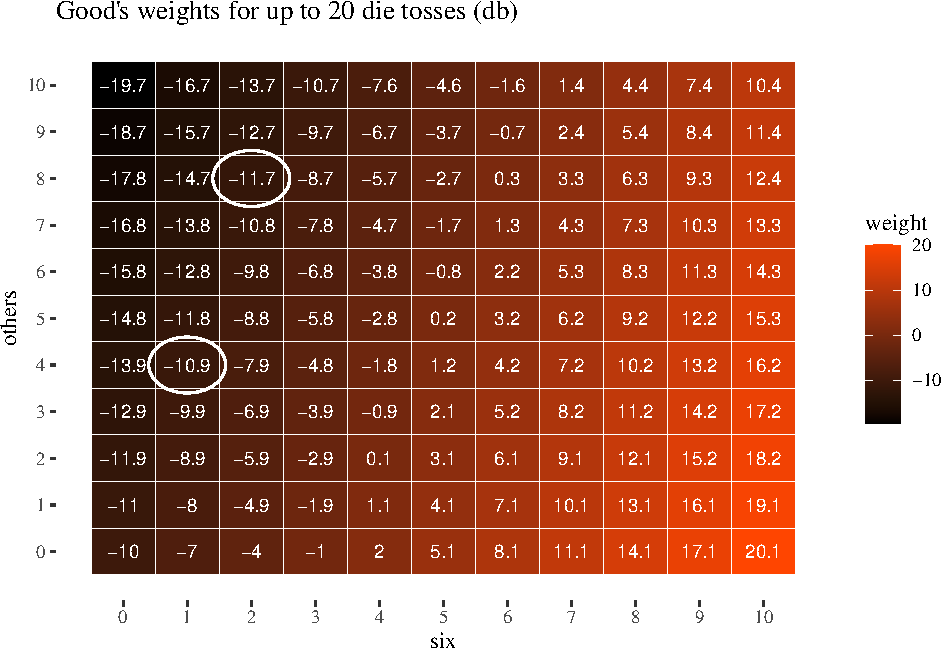
\includegraphics[width=1\linewidth]{imprecision_weight_files/figure-latex/goodWEights-1} \end{center}
\caption{Good's weights in dbs, rounded, for all possible outcomes of up to 20 tosses of a die randomly selected from 10 dice nine of which were fair, and one is \nicefrac{1}{3} loaded towards six. $H=$`the die is loaded'.}
\label{fig:goodWeight}
\end{figure}

Two facts are notable. (1) Weight can drop with sample size: for
instance the weight for 4 others and 5 sixes is 1.2db, and it is .2db
for 5 others and 5 sixes. (2) Weight can drop while the sample size
increases even if the proportion of sixes remains the same. For
instance, if none of the observations are sixes, the weights go from -10
to -19.7 as the sample size goes from 0 to 10. Less trivially, the
observation of one six in five leads to weight of -10.9, while the
observation of two sixes in ten tosses leads to weight -11.7. That is,
(Monotonicity), (Completeness), (Weak increase) and (Strong increase)
all fail for Good's measure.

Moreover, there is a conceptual difficulty in the neighborhood. Suppose
you are trying to ascertain the bias \(\theta\) of a coin, but you do
not restrict yourself to two hypotheses as in the dice example, but
rather initially take any bias to be equally likely. For each particular
hypothesis \(\theta = x\) and any set of observations \(E\) you can use
the binomial distribution to calculate \(\pr{E \vert \theta = x}\). But
to deploy Good's definition, you also need
\(\pr{E \vert \theta \neq x}\), which is less trivial, as now you have
to integrate to calculate the expected probability of the evidence given
an infinite array of possible values of \(y\). Suppose you have no
problem calculating such items. Now imagine you observe 10 heads in 20
tosses. The question `how weighty is the evidence' makes no sense here,
as Good's weight needs a hypothesis (and its negation) to be plugged in.
For this reason, in such a situation, we can at best talk about a
continuum of Good's weights, one for each particular value of
\(\theta\).

\begin{itemize}
\item
  compare to pointwise mutual information
\item
  evaluate in light of the desiderata
\end{itemize}

\hypertarget{weight-and-completeness}{%
\section{Weight and completeness}\label{weight-and-completeness}}

A question similar to ``how weighty is the evidence'' is ``how complete
is it''? These are conceptually different: the former asks about how
much information pertinent to a given hypotheses the evidence provides,
or, about the amount of evidence relevant to that hypothesis, the latter
seems to suggest a comparison to some ideal list of what such items
would be needed for the evidence to be complete. While we think that
these notions, albeit related, should be clearly distinguished, the
distinction has not always been made clearly in the literature, starting
with Keynes himself, who suggested that in their evaluation of the
evidence an agent should consider ``the degree of completeness of the
information upon which a probability is based.'' {[}TP
p.~345{]}\todo{REF}

This picture of ideal-list-of-evidence-relative notion of weight has
been explored by {[}CITE FEDUZI 2010{]}. \todo{CITE NANCE HERE?} Let us
first present the view following {[}CITE FEDUZI 343{]}, \(\Omega\)
stands for the set of all items of possible evidence relevant for
estimating the probability of the hypothesis \(H\). Let \(K\) be the
agent's knowledge, the set of items of evidence already obtained by the
agent, \(K \subseteq \Omega\). Then her relevant ignorance is
\(I = \Omega \setminus K\).

Then, Feduzi, following {[}CITE RUNDE 1990{]}, proposes to define the
weight of information \(E\) provides about \(H\), \(V(H/E)\) as follows:
\begin{align} \tag{Vdiv}  V(H/E) & = \frac{K}{K+I}.\end{align}
\noindent While literally it does not make sense to divide sets by sets,
we might charitably interpreting Feduzi as using \(\Omega, K\) and \(I\)
the symbols ambiguously, standing for both the sets of items of
evidence, and the amount of relevant information that the sets contain.
The obvious difficulty is that it is not a successful explication (at
least not yet), as we are not told how to get \(K\) and \(K+I\) as
numerical values to be used in the division. But however we get them,
let us see whether (Vdiv) can result in any insights.

First, one advantage of the completeness approach is that the resolution
of the stopping problem is more or less automatic: the agent should make
the decision if the evidence is complete, and should collect more
evidence if it is not. Later on, when discussing Nance's approach to the
notion, we will see a complication: obtaining further evidence might be
practically unfeasible, and so it makes sense to distinguish ideal
completeness from reasonable completeness and base the practical
stopping rule on the former. For now, we put this complication aside.

Second, it might be the case that obtaining further evidence while
providing more information results in the decrease of weight. Here is an
example illustrating this due to Feduzi {[}CITE 345{]}. Joan in her
research tries to establish who is the most quoted author in the
literature on decision theory under ambiguity. \(\Omega\) is the set of
all \(n\) papers (though of as items of evidence \(E_1, \dots, E_n\)).
\(K_0\) contains the \(m\) papers that Joan inspected so far
(\(E_1, \dots, E_m\), \(m<n\). \(I_0\) is the set of papers she did not
look at yet, \(\Omega = K_0 \cup I_0\). However, Joan is aware only of a
part of \(\Omega\), the papers in the field she believes exist, \(S\).
Thus, her objective ignorance, \(I_0\), and her subjective ignorance,
\(I_S = S- K\), diverge, as she underestimates the amount of papers that
she has not yet encountered. Joan's assessment of weight is going to be
\(\nicefrac{K}{K+I_s}\). Say Joan formulates a hypothesis, \(H\):
``Ellsberg is the most highly cited author in the ambiguity literature''
and that she is quite confident that the papers she had not looked at
yet would not significantly affect the probability of \(H\). She thinks
she has read enough, say \(\pr{H \vert K} = .7\) and \(V(H/K) = .8\).
Then, she looks at another paper, somewhat increasing \(K\), but that
paper contains reference to many papers she has not heard of in journals
that she has not heard of, thus increasing her estimation of \(S\) quite
a lot--- the ultimate impact of the new evidence is a drop in weight as
the denominator in (Vdiv) will grow much more than the numerator. Thus,
(Monotonicity) \todo{check crossref} can fail on this approach.

However, even putting the conceptual difference between weight and
completeness that we have already mentioned aside, there are concerns
about using degrees of completeness as our explication of the notion of
weight of evidence.

To start with, we have not really explicated the notion of the amount of
evidence employed in (Vdiv). Sure, we could simply count propositions.
One simple strategy, to be used if we do not want to use (Vdiv) would be
to simply count the relevant propositions included in the
evidence---this would validate (Monotonicity) \todo{check crossref}.
Another strategy along these lines would be to assign sizes to sets of
propositions and use these as numbers in (Vdiv), invalidating
(Monotonicity) in the process. Either way, the strategy is not viable,
as it is too syntax-sensitive. Different propositions, intuitively, can
contain hugely different amount of nevertheless relevant information
\todo{is this trivial or do we need an example?}, and the individuation
of propositions is too arbitrary a matter to take such an approach
seriously. On one hand, without some measure of assigning numerical
values to sets of evidence, we have no way to deploy (Vdiv). On the
other hand, if we could meaningfully assign numbers expressing the
``amount of evidence'' prior to any application of (Vdiv), there are no
clear reasons why we should take these number to express weights of
evidence, especially given the second concern with the completeness
approach.

So the second difficulty is that on this approach the weight of evidence
becomes very sensitive not only to what the actual evidence is, but also
to what an ideal evidence in a given case should be. unless as clear and
epistemologically principled guidance as to how to formulate such ideal
lists is available, this seems to open a gate to arbitrariness. Change
of awareness of one's own ignorance, without any major chance to the
actual evidence obtained, might lead to overconfidence or
under-confidence in one's judgment. Moreover, it is not clear how
disagreement about weight arising between agents not due to evidential
differences, but rather due to differences in their list of ideal items
of evidence should be adjudicated.

\hypertarget{skyrms-and-resilience}{%
\section{Skyrms and resilience?}\label{skyrms-and-resilience}}

\begin{itemize}
\tightlist
\item
\item
  relation to law Davidson Pargetter 1986, perhaps Nance, who else?
\end{itemize}

\hypertarget{evidential-probability-and-weight}{%
\section{Evidential probability and
weight}\label{evidential-probability-and-weight}}

{[}PEDDEN 2018{]} \todo{REF} follows a suggestion from {[}KYBURG
1961{]}\todo{REF Kyburg. Probability and the Logic of Rational Belief. Wesleyan University Press, Mid-
dletown Connecticut, 1961 and H. E. Kyburg and C. M. Teng. Uncertain Inference. Cambridge University Press, Cam-
bridge, 2001.} He proposed using the degree of imprecision of the
intervals in his probability system called Evidential Probability (EP).
The key idea in EP is that evidential probabilities should be imprecise,
and so accordingly an evidential probability function \(\mathsf{EP}\) is
of the form \(\mathsf{EP}(H \vert E \wedge K) = [x,y]\), where the
right-hand is the closed interval expressing the objective degree of
support that \(E\wedge K\) provide for \(H\).

How is this interval to be determined, though? Kyburg's proposal is the
following, if the hypothesis is about a single object \(o\) and a
predicate \(P\). For the reference classes to which \(o\) is known to
belong and for which \(K\) contains frequency information (possibly
imprecise, in the interval form) for objects with \(P\), enumerate the
corresponding frequency statements, \(r_1, \dots, r_n\). Now, you are
facing a reference class problem. Apply sequentially the following
rules:

\begin{tabular}{lp{10cm}}
(Sharpening by richness) & If $r_j$ conflicts with $r_i$ and $r_i$ has been obtained from a marginal distribution while $r_j$ from a full joint distribution, ignore $r_i$. 
\end{tabular}

As the formulation might be somewhat cryptic, let us illustrate the
recommendation with an
example.\todo{make sure these examples are better made sense of the HOP way!}

\begin{tabular}{lp{10cm}}
(Richness example) &suppose you are drawing a card from one of two decks of cards, $H:=$ `you will draw the Ace of Spades'. You know that Deck 1 is a regular deck, and Deck 2 is a regular Deck with the Ace of Spades removed. First you toss a fair die and use Deck 1 if the die lands on 1 or 2, and use Deck 2 otherwise. You have at least two frequencies to consider:
\begin{itemize}
\item The frequency of Aces of Spades in the total number o cards ($\nicefrac{1}{103}$), which is your marginal-distribution-based-probability.
\item The one obtained by using the information about the die, and about the frequencies in the decks. There is probability $\nicefrac{1}{3}$ of using Deck 1 which is the only deck containing the card, in which the probability of drawing it is $\nicefrac{1}{52}$, so the probability to be used is $\nicefrac{1}{3}\nicefrac{1}{52}= \nicefrac{1}{156}$.
\end{itemize}
\end{tabular}

One can easily observe that \(\nicefrac{1}{103}\) simply is not the
probability of drawing the Ace of Spades in the setup. After all, we are
not drawing a random card from the joint decks, but have to factor in
the uneven probabilities of the decks being chosen, and once we do so,
the correct probability is \(\nicefrac{1}{156}\). The second strategy is
this:

\begin{tabular}{lp{10cm}}
(Sharpening by specificity) & If among the remaining intervals $r_j$ conflicts with $r_i$ and $r_j$ is a proper subset of $r_i$, choose $r_j$ over $r_i$.
\end{tabular}

\noindent This mirrors the idea that one should use more specific
information. The third rule is:

\begin{tabular}{lp{10cm}}
(Sharpening by precision) & If there is a single interval that is a proper sub-interval  of every other interval, this is the evidential probability. Otherwise, the evidential probability is the shortest possible cover of these intervals.
\end{tabular}

With this system in the background, {[}PEDDEN 2018 681{]} proposes the
following definition of the weight of the argument for \(H\) given \(E\)
and \(K\), where \(\mathsf{EP}(H \vert E \wedge K) = [x,y]\):
\begin{align}
\tag{WK} & \mathsf{WK(H\vert E\wedge K)} & = 1 - (y-x)
\end{align} That is, the weight of the evidence is the spread of the
evidential probability, transformed to scale between 0 and 1, reaching 1
when the spread is 0 and 0 when the spread is 1.

How is this approach to be applied to examples such as the one by C. S.
Peirce (recall: drawing balls with replacement from an urn, with
observed frequency of white balls .5, in one scenario the sample size is
1000 in another it is 2)?

{[}PEDDEN 2018 686{]} proposes the following analysis, of an example
analogous to that by Peirce. You are drawing from an urn full of black
and red beans (the proportion is unknown). First, abbreviations:

\begin{tabular}{lp{10cm}}
$H$ & $49.5-50.5\%$ of the beans are red. \\
$E_1$ & 2 sampled beans are red. \\
$E_2$ & 3000 sample beans are red. 
\end{tabular}

\noindent Further, imagine you have enough information to calculate that
between \(2\%\) and \(100\%\) of two-fold samples of any large finite
population will be matching samples, that is they will match the
population with a margin of error of \(1\%\). Then
\(\mathsf{EP}(H \vert E_1 \wedge K) = [.02, 1]\). Similarly, Pedden
invites us to suppose that we can calculate the relative frequency of
3000-fold samples that match any large finite population within a margin
of error of \(1\%\) to somewhere between \(72.665\%\) and \(100\%\), so
accordingly \(\mathsf{EP}(H \vert E_2 \wedge K) = [.72665, 1]\). Then,
the corresponding values of \(\mathsf{WK}\) are .02 and .72665 (this is
because in both cases \(y =1\) and \(1 - (1 -x) = x\)).

What are we to make of this? Are imprecise probabilities promising when
it comes to the explication of weight of evidence? Some progress has
been made, but note the following limitations.

\begin{itemize}
\item
  The edges of the intervals are what contributes to \textsf{WK}. They
  are highly sensitive to the choice of the margin of error, but what
  margin of error to choose and why remains a mystery, and what margin
  of error has been chosen does not function anywhere in the
  \(\mathsf{EP}\) representation of uncertainty.
\item
  Relatedly, it may easily happen that for two different distributions
  the \(1\%\) intervals will be identical while the 78\%\$ intervals
  will not. Such differences will obviously not be captured by the 1\%
  margin of error intervals.
\item
  The calculations of such intervals might be easy for simple
  combinatorial cases, but it is far from obvious how similar intervals
  are to be obtained for more complicated real-life cases. Emphatically,
  classical statistical confidence intervals are not ranges within which
  the true parameter lies with a certain probability (and if you
  interpret confidence intervals this way, you behave as if you were
  running a Bayesian reasoning with a uniform prior, which is often
  unjustified and prone to over-fitting).
\end{itemize}

Before we abandon the idea, though, let us know that over the last 30
years we have observed a revival of imprecise probabilities, and so it
is only fair that we should take its most recent versions for a ride.
Hence our next interest: imprecise probabilism, its motivations, the
difficulties it runs into.

\hypertarget{imprecise-probabilities-and-weight}{%
\section{Imprecise probabilities and
weight}\label{imprecise-probabilities-and-weight}}

The point of departure for imprecise probabilism (\textsf{IP}) is the
precise probabilism (\textsf{PP}), which we are already familiar with.
On the latter view, a rational agent's uncertainty is to be represented
as a single probability measure. \textbf{Imprecise probabilism}, in
contrast with PP, holds that an agent's credal stance towards a
hypothesis \(H\) is to be represented by means of a set of probability
measures, called a representor, \(\mathbb{P}\), rather than a single
measure \(\mathsf{P}\). The idea is that the representor should include
all and only those probability measures which are compatible with this
evidence. For instance, if an agent knows that the coin is fair, their
credal stance would be captured by \(\{\mathsf{P}\}\), where
\(\mathsf{P}\) is simply a probability measure which assigns \(.5\) to
\(H\). If, on the other hand, the agent knows nothing about the coin's
bias, their stance would rather be represented by means of the set of
all probabilistic measures, as none of them is excluded by the available
evidence. Note that on IP it is not the case that the set represents
admissible options and the agent can legitimately pick any precise
measure from the set. Rather, the agent's credal stance is essentially
imprecise and has to be represented by means of the whole
set.\footnote{For the development of IP see (Fraassen, 2006; Gärdenfors
  \& Sahlin, 1982; Joyce, 2005; J. Kaplan, 1968; Keynes, 1921; Levi,
  1974; Sturgeon, 2008; Walley, 1991), (Bradley, 2019) is a good source
  of literature.} The literature contains an array of arguments for IP.
Let us take a look at the main ones.

\begin{itemize}
\item
  \textsf{PP} does not seem appropriately evidence-responsive,
  especially when evidence is limited. Following \textsf{PP}, in
  Peirce's example, the agent's uncertainty about \(W:=\)``the next
  drawn ball is going to be white' is \(.5\) no matter whether you have
  drawn two balls one of which was white, or a thousand balls, five
  hundred of which were white.
\item
  Indifference is not sensitive to sweetening (improving the chances of
  \(H\) only slightly), while \textsf{PP} predicts such sensitivity. For
  instance, if you do not know what the bias of a coin is, learning that
  it now has been slightly modified to increase the probability of heads
  by .001 will still leave you unwilling to bet on heads in a bet that
  would've been fair if the actual chance of \(H\) was .5 and not .001.
\item
  \textsf{PP} has problems representing complete lack of knowledge.
  Suppose you start tossing the coin starting with knowing only that the
  coin bias is in \([0,1]\) and then observe the outcome of ten tosses,
  half of which turn out to be heads. This is some evidence for the real
  bias being around .5. How do you represent your stances before and
  after the observations? If you deploy the principle of insufficient
  evidence, you start with \(\mathsf{P}_0(H)=.5\) and end with
  \(\mathsf{P}_1(H)=.5\), as if nothing changed. If you do not deploy
  the principle of insufficient evidence, what do you do?
\item
  \textsf{PP} has problems with formulating a sensible method of
  probabilistic opinion aggregation Stewart \& Quintana (2018). A
  seemingly intuitive constraint is that if every member agrees that
  \(X\) and \(Y\) are probabilistically independent, the aggregated
  credence should respect this. But this is hard to achieve if we stick
  to PP (Dietrich \& List, 2016). For instance, a \emph{prima facie}
  obvious method of linear pooling does not respect this. Consider
  probabilistic measures \(p\) and \(q\) such that
  \(p(X) = p(Y) = p(X\vert Y) = 1/3\) and
  \(q(X) = q(Y) = q(X\vert Y) = 2/3\). On both measures, taken
  separately, \(X\) and \(Y\) are independent. Now take the average,
  \(r=p/2+q/2\). Then \(r(X\cap Y) = 5/18 \neq r(X)r(Y)=1/4\).
\end{itemize}

One key difference between Kyburg's \textsf{EP} and \textsf{IP} is that
on the latter we use sets of probability measure instead of intervals.
This makes the approach not only more general (as now, for instance, the
resulting probabilities of a proposition in question do not have to form
a closed interval), but also provides a more general and less
idiosyncratic picture of learning from evidence, that is a a natural
extension of the classical Bayesian approach. When faced with new
evidence \(E\) between time \(t_0\) and \(t_1\), RA's representor should
be updated point-wise, running the standard Bayesian updating on each
probability measure in the representor:
\begin{align*} \label{eq:updateRepresentor}
\mathbb{P}_{t_1} = \{\mathsf{P}_{t_1}\vert \exists\, {\mathsf{P}_{t_0} \!\in  \mathbb{P}_{t_0}}\,\, \forall\, {H}\,\, \left[\mathsf{P}_{t_1}(H)=\mathsf{P}_{t_0}(H \vert E)\right] \}.
\end{align*}

How is weight of evidence to be measured on \textsf{IP} (Joyce, 2005; M.
Kaplan, 1996; Sturgeon, 2008)? One line, analogous to the one taken by
Pedden is to take the edges of the resulting interval that captures
changes in the weight of evidence (Walley, 1991). If you know the
proportion of beans is between .02 and 1, your interval is wider than it
is if you know the proportion is between 0.72665. In this sense, this
approach, admittedly, handles cases such as the beans example.

The main question here, though, is that it is not clear how you are
supposed to learn that the proportion of beans is such and such. This is
related to the problem of belief inertia (Levi, 1980). Say you start
drawing beans knowing only that the true proportion of red beans is in
\((0,1)\) and then draw two beans both of which are red. On \textsf{IP}
your initial credal state is to be modeled by the set of all possible
probability measures over your algebra of propositions. Once you observe
the two beans, each particular measure from your initial representor
gets updated to a different one that assigns a higher probability to
``red'', but also each measure in your original representor can be
obtained by updating some other measure in your original representor on
the evidence (and the picture does not change if you continue with the
remaining 2998 observations) . Thus, if you are to update your
representor point-wise, you will end up with the same representor set.
Consequently, the edges of your resulting interval will remain the same.

Relatedly, recall that the main selling point for \textsf{IP} was its
ability to account for how credal states are responsive to the evidence
and the amount thereof. But it is not clear how to make sense of
evidential constraints in a way that makes them go beyond testimonial
evidence. On \textsf{IP} the representors are somehow to obey the
evidential constraints: they are supposed to be point-wise updated on
the evidence, and to contain only those probabilistic measures that are
not excluded by the evidence obtained so far. But how exactly does the
evidence exclude probability measures? This is not a mathematical
question: mathematically (Bradley, 2012), evidential constraints are
fairly easy to model, as they can take the form of the
\emph{evidence of chances} \(\{ \mathsf{P}(X) = x\}\) or
\(\mathsf{P}(X) \in [x,y]\), or be \emph{structural constraints} such as
``\(X\) and \(Y\) are independent'' or ``\(X\) is more likely than
\(Y\).'' While it is clear that these constraints are something that an
agent can come to accept if offered such information by an expert to
which the agent completely defers, it is not trivial to explain how
non-testimonial evidence can result in such constraints.

Most of the examples in the literature start with the assumption that
the agent is told by a believable source that the chances are
such-and-such, or that the experimental set-up is such that the agent
knows that such and such structural constraint is satisfied. But outside
of such ideal circumstances what observations exactly would need to be
made to come to accept such constraints remains unclear. And the
question is urging: even if you were lucky enough to run into an expert
that you completely trust that provides you with a constraint like this,
how exactly did the expert come to learn the constraint? The chain of
testimonial evidence has to end somewhere!

Admittedly, there are straightforward degenerate cases: if you see the
outcome of a coin toss to be heads, you reject the measure with
\(\mathsf{P}(H)=0\), and similarly for tails. Another class of cases
might arise if you are randomly drawing objects from a finite set where
the real frequencies are already known, because this finite set has been
inspected. But such extreme cases aside, what else? Mere consistency
constraint wouldn't get the agent very far in the game of excluding
probability measures, as way too many probability measures are strictly
speaking still consistent with the observations for evidence to result
in epistemic progress.

Bradley suggests that ``statistical evidence might inform
{[}evidential{]} constraints {[}\dots and that evidence{]} of causes
might inform structural constraints'' {[}125-126{]}. This, however, is
far cry from a clear account of how exactly this should proceed. Now,
one suggestion might be that once a statistical significance threshold
is selected, a given set of observations with a selection of background
modeling assumptions yields a confidence interval, and perhaps that the
bounds of this confidence interval should be the lower and upper
envelope---this is in line with the example used by Pedden (and our
objections to such a use of conidence intervals apply here as well).
Moreover, notice that whatever problems Bayesian statisticians raise
against classical statistics apply here. To mention a few: the approach
uses MLE and so is not sensitive to priors (or, in other words, is
equivalent to always taking maximally uninformative priors), the
estimates are sensitive to stopping intention, and there are no clear
methods for combining various pieces of information of this sort (if
this was easy, there would be no need for meta-analysis in statistical
practice).\footnote{Admittedly, there are formulae for calculating confindence intervals based on two confidence intervals if they are based on separate independent observations in an experiment of exactly the same design, but this is a very idealized setup.}

Even supposing that a sensible mechanism of the exclusion in question
has been proposed, measuring weight along the lines of (WK) or by the
absolute distance between the edges of the interval has a weakness we
already signaled. It is a function of two points and is completely
insensitive to what happens between them. If we are looking at a
somewhat monolithic class of distributions, say all beta distributions,
looking at where the 1st and the 99th centiles are located might be a
good rough guide to what is happening in between. But without such a
restriction, not so much.

Here is an example of how easily more complicated cases that could be
misrepresented by looking only at the envelopes might arise. Suppose you
start with knowing that the coin bias lies within \((.4, .6)\)
(Situation A). Then you hear from two equally reliable witnesses: one
tells you that the real bias is exactly .4 and the other one tells them
the real bias is exactly .6 (Situation B). It seems that you now have
more evidence than before, but it is unclear how this difference is to
be captured by the edges of the interval of non-excluded values, as the
edges are exactly the same.

Another stab at explicating weight of evidence within the \textsf{IP}
framework has been made by Joyce (2005). Joyce uses a density over
chance hypotheses to account for the notion of evidential weight. He
conceptualizes the weight of evidence as an increase of concentration of
smaller subsets of chance hypotheses: \begin{align}
\tag{Joyce} w(X,E) & = \sum_x \vert c(ch(X) = x  \vert E) \times (x - c(X\vert E))^2 - c(ch(X) = x) \times (x - c(X))^2\vert
\end{align}

\noindent This looks a bit complicated, so let us take this slow.
Suppose you only consider three chance hypotheses, that the coin bias is
one of \(.4, .5,\) and \(.6\), that is, the hypotheses are
\(ch(X) = .4, ch(X)=.5,\) and \(ch(X)=.6\). For each
\(x\in \{.4, .5, .6\}\)) you attach a prior credence \(c(ch(X) = x)\) to
the corresponding hypothesis. Say you start with equal priors, that is
for all \(x\in \{.4, .5, .6\}\) you have
\(c(ch(X) =x) = \nicefrac{1}{3}\). Then, your expected value of \(X\),
which Joyce takes to be your credence in \(X\) simpliciter is
\(\sum_x c(Ch(X)=x)x\), which is .5.

Now consider your evidence: you tossed the coin and observed, say, seven
heads out of ten tosses. We need \(c(ch(X)=x \vert E)\). By Bayes, we
have: \begin{align*}
c(ch(X)=x \vert E) & = \frac{c(E \vert ch(X) =x) c(ch(X)=x )}{c(E)},
\end{align*} \noindent so we need to calculate the likelihoods,
\(c(E \vert ch(X) =x)\). We assume you are probabilistically coherent,
that you defer to chances, and know the experimental setup, so that the
likelihoods are calculated using the binomial distribution, i.e.~if the
evidence is \(a\) heads and \(b\) tails: \begin{align*}
c(E \vert ch(X) =x) & = {a+b \choose a}\,x ^a (1-x)^{b}
\end{align*} \noindent In our example, the likelihoods (rounded) are
\(.042, .117\), and \(.214\) respectively. The denominator is calculated
by taking \(c(E) = \sum_x c(E \vert ch(X) =x) c(ch(X)=x)\), which in our
case turns out to be \(.124\). Putting these together, the values of
\(c(ch(X)=x \vert E)\) are \(.113\) \(.312\), and \(.573\) (rounded).
Then, your expected value, which Joyce to be your credence in \(X\)
simpliciter conditional on \(E\) is \(\sum_x c(Ch(X)=x\vert E)x\), which
is \(.54\).

Once that we went over an example illustrating the quantities employed
in (Joyce), before we plug these into the final formula, let us try to
understand Joyce's motivations for such an explication. The idea here is
that weighty evidence should make the credence resilient, and resilience
makes the difference between the posterior credence in chances
\(c(ch(X)=x \vert E)\) and the prior credence in chances \(c(ch(X)=x)\).
The complication is that the impact of this difference should be lower
for for those values of \(x\) that are close to \(c(X\vert E)\) for the
posterior and close to \(c(X)\) for the prior. Hence, the formula for
\(w\) is takes (the absolute value of) the difference between posteriors
and priors weighed by, these (squared) distances. The weightier the
evidence, the smaller \(w\) is supposed to be.

Accordingly, in our example the weights for the prior are
\(-.1^2, 0, .1^2 = 0.01, 0, .01\), the weights for the posterior are
\(.021330539, .002120582\), and \(.0029\) and w is \(0.003241822\). For
comparison, if instead we observed 70 heads in 100 tosses, \(w\) would
be \(.006689603\).

There are various issues with this approach. One is that now to evaluate
the weight of evidence \(E\) with respect to proposition \(X\) now you
need to have and use in your calculations your estimation of chances of
\(X\). Let us put aside the worry that it is not obvious that we can
meaningfully talk about chances of arbitrary propositions. Even then,
the name of the game for the imprecise probabilist was to express the
uncertainty about \(X\) in terms of a representor, a set of probability
measures. However, one can have a representor with respect to a set of
object-level propositions including \(X\) without having a single
credence about chances, so now the calculations of weight of \(E\) with
respect to \(X\) do not fall out whatever was supposed to capture the
agent's uncertainty about \(X\), \(E\) and their relationship.

Moreover, the reader might have observed that the values of \(w\) for
our example are not very telling. A ten-fold increase in sample size,
with frequency being fixed, results in \(w\) dropping by \(62\%\), and
both are small numbers that are hard to interpret. This raises the
question: how does the measure behave with respect to binomial trials
and are the outcomes intuitively acceptable? Let us take the measure for
a ride.

First, suppose we keep the same priors, and calculate \(w\) depending on
how many successes we have observed in the 10 tosses. The results are as
follows:

\begin{figure}

\begin{center}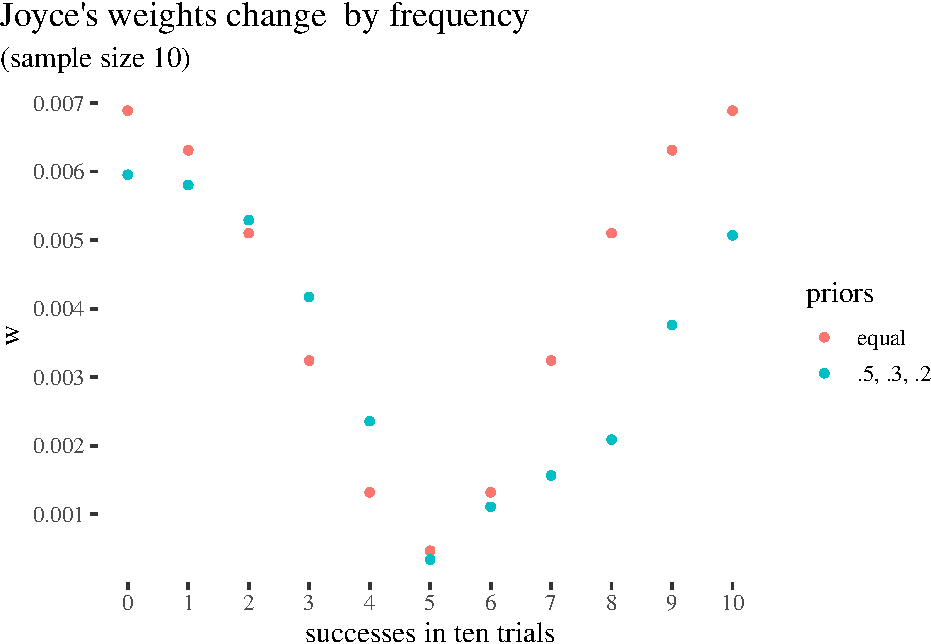
\includegraphics[width=1\linewidth]{imprecision_weight_files/figure-latex/joyce1-1} \end{center}

\caption{Joyce's $w$ (the lower it is, the higher the weight) for various observed successes in 10 Bernoulli trials. Three chance chypotheses: $.4, .5, .6$, and two sets of priors: equal and $.5, .3, .2$ respectively. Note how the weightiest evidence is obtained with five observed successes and how its drop is fourteen-fold, if the observed frequency is 0.}
\label{fig:joyce1}
\end{figure}

The behavior of \(w\) is even more unusual if the sample size is higher.
In Figure \ref{fig:joyce2} we illustrate what happens with \(n=100\),
for various possible outcomes of 100 Bernoulli trials.

\begin{figure}

\begin{center}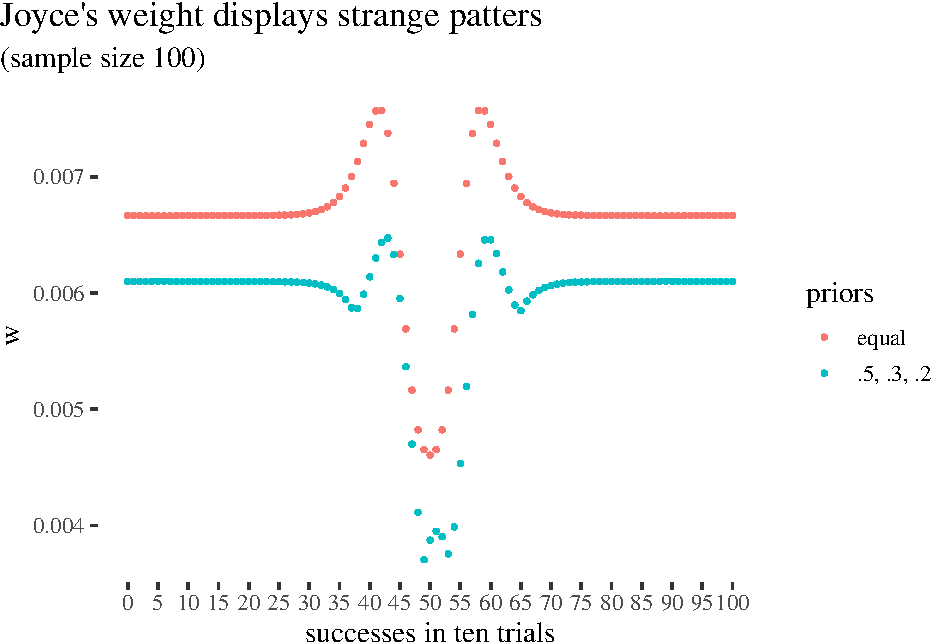
\includegraphics[width=1\linewidth]{imprecision_weight_files/figure-latex/joyce2-1} \end{center}

\caption{Joyce's $w$ (the lower it is, the higher the weight) for various observed successes in 100 Bernoulli trials. Three chance chypotheses: $.4, .5, .6$, and two sets of priors: equal and $.5, .3, .2$ respectively. Agan, the weightiest evidence is obtained with successes close to the expected value, with  large variation for observed frequencies not too far from the expected values, fairly flat otherwise.}
\label{fig:joyce2}
\end{figure}

So this measure might result in drastic shift in weights even if the
observed frequenciesa are not too far from the chance hypotheses. This
we find undesirable.

In Figure \ref{fig:joyce3} we illustrate two other phenomena, which
might come up when the observed frequencies are kept fixed, but the
sample size increases.

\begin{figure}

\begin{center}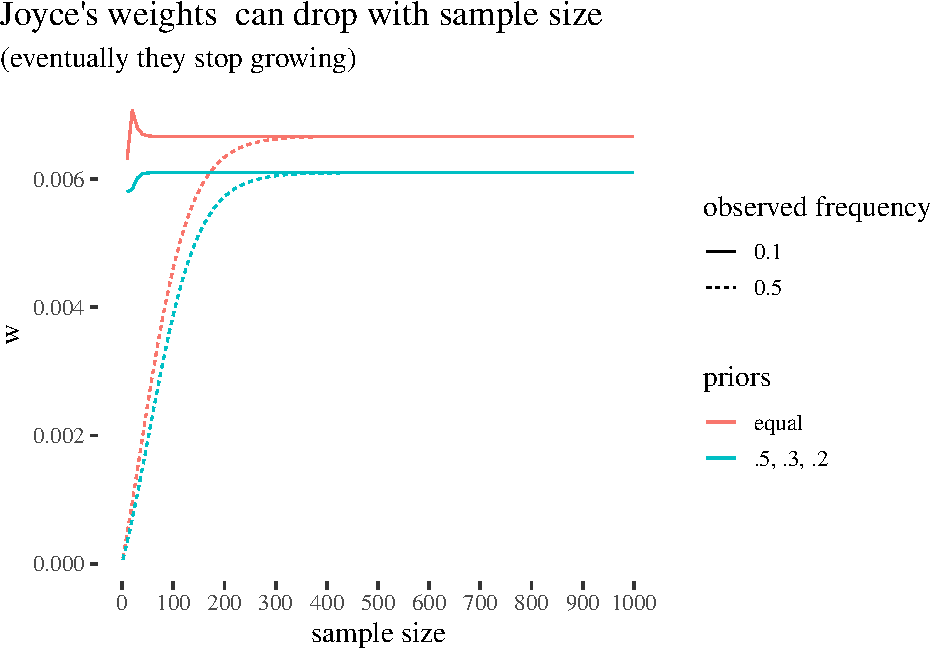
\includegraphics[width=1\linewidth]{imprecision_weight_files/figure-latex/joyce3plot-1} \end{center}

\caption{Joyce's $w$ (the lower it is, the higher the weight) for two fixed success ratio across various observed successes in  Bernoulli trials (lines are used for smoothing).  Note large shifts with possible decrease in the beginning, and a flattening afterwards.}
\label{fig:joyce2}
\end{figure}

What is the reason for this strange behavior? The shapinig of Joyce's
weight is a balancing act. For instance, for frequency .1 with equal
priors the weight is maximized at \(n=90\) and starts dropping at
\(n=100\). Why? We start with three chance hypotheses, \(.4, .5, .6\)
with equal priors. Once the observations have been made, the posterior
for the chance hypotheses is focused at the chance hypothesis .4 (its
posterior is more or less .99999), and so is the credence in \(X\)
simpliciter (this expected value is .4000003). Now the weights are build
by measuring square distance from the credence in \(X\) simpliciter and
since the expected value is nearly equal to the lowest chance hypothesis
under consideration, the weight for the lowest chance hypothesis is
\(8.260660e-14\), so while the posterior for this hypothesis is very
high, the weight is very low and its contribution to the weight
calculation is severely limited. Ultimately, what happens with weight is
now a matter of balancing the uneven posteriors with squared penalties
(or rewards, really) for the distance from the expected value (which is
pretty much the most likely hypothesis once you have made enough
observations). Once you observe 10 successes in 1000 trials, the
credence in \(X\) simpliciter becomes \(.4000001\), so the distance of
the lowest chance hypothesis to it drops, and this weight drops
``faster'' than the resulting increase in the probability of the lowest
chance hypothesis itself. The stabiliziation is achieved because further
on the posterior for this hypothesis can only get closer to one (and
closer to zero for all the other hypotheses).

Moreover, this approach is of limited applicability. For one thing, as
Joyce admits, it is supposed to work when RA's credence is mediated by
chance hypotheses. Depending on applications, such a mediation might be
unavailable. Another issue is that this might work for unimodal
distributions when we only consider the influx of new data points, but
it's unlikely to give desired results if, say, the evidence obtained is
the testimony of disagreeing witnesses. This is because an essential
part of the calculations relies on taking the expected value, and it is
not too hard to imagine cases of diverging items of evidence resulting
only in a small chance of the expected value.
\todo{Should I further elaborate?}

The approach insists that an agent's stance towards a proposition should
be represented as the expected value of the chance hypothesis---and we
will argue against this view later on. At this point, what is crucial
for us, the proposal employs probabilities or probability densities (if
we go continuous) over parameter values. Even if we do not assume these
are chances and treat them as, say, parameters that are potentially
rational to accept in light of the evidence, by using this approach we
no longer can represent uncertainty about a proposition in terms of a
set of probability measures over any algebra containing the proposition
itself (as the algebra now also needs to contain the chance hypotheses
as well!). Perhaps, this is as it should be. But then, as I will argue
later one, there are useful ways to go this way without turning to
IP---after all, notice how the notion of a representor plays no role in
Joyce's explication of weight whatsoever!

\hypertarget{troubles-with-imprecise-probabilism}{%
\section{Troubles with imprecise
probabilism}\label{troubles-with-imprecise-probabilism}}

The interval-based \textsf{IP} approach to weight of evidence runs into
two specific problem: insensitivity to what happens between the edges,
and sensitivity to risk-related decisions made which are not even
represented in \textsf{IP}'s preferred uncertainty representation
methods. There are however more general problems with \textsf{IP}, which
suggest we should move on, and to some extent the direction in which we
should do so.

\begin{itemize}
\item
  \textsf{IP} has no means of distinguishing the situation in which you
  are about to toss a coin whose bias is either .4 or .6., and the one
  in which you are about to toss a coin whose bias is also either .4 or
  .6,, but the bias .4 is three times more likely than .6, at least not
  without moving to higher-order probabilities, in which case it is no
  longer clear whether the object-level imprecision performs any
  valuable task.
\item
  if one decides to favor \textsf{IP} over \textsf{PP} because
  \textsf{PP} involves seemingly artificial precision, such artificial
  precision can't be avoided by moving to IP (Carr, 2020). Take the
  well-known Jellyfish example (Elga, 2010): I'm pulling stuff out of my
  purse, there seems to be no rule as to what I have pulled out so far,
  how likely is it that the next thing I pull out will be a jellyfish?
  The impreciser is committed to there being a precise \emph{range} of
  probabilities to be assigned to the jellyfish hypothesis. Say it's
  \([.2-.8]\). But why this rather than, say \([.2,.80001]\)?
\item
  \textsf{IP} gives wrong comparison predictions (Rinard, 2013). Suppose
  you know of two urns, \textsf{GREEN} and \textsf{MYSTERY}. You are
  certain \textsf{GREEN} contains only green marbles, but have no
  information about \textsf{MYSTERY}. A marble will be drawn at random
  from each. You should be certain that the marble drawn from
  \textsf{GREEN} will be green (\(G\)), and you should be more confident
  about this than about the proposition that the marble from
  \textsf{MYSTERY} will be green (\(M\)). In line with how lack of
  information is to be represented on \textsf{IP}, for each
  \(r\in [0,1]\) your representor contains a \(\mathsf{P}\) with
  \(\pr{M}=r\). But then, it also contains one with \(\pr{M}=1\). This
  means that it is not the case that for any probability measure
  \(\mathsf{P}\) in your representor, \(\mathsf{P}(G) > \mathsf{P}(M)\),
  that is, it is not the case that RA is more confident of \(G\) than of
  \(M\). This is highly counter-intuitive.
\item
  \textsf{IP}, as already mentioned, faces belief inertia. Here's
  another example from (Rinard, 2013). Either all the marbles in the urn
  are green (\(H_1\)), or exactly one tenth of the marbles are green
  (\(H_2\)). Your initial credence \([0,1]\) in each. Then you learn
  that a marble drawn at random from the urn is green (\(E\)). After
  conditionalizing each function in your representor on this evidence,
  you end up with the the same spread of values for \(H_1\) that you had
  before learning \(E\), and no matter how many marbles are sampled from
  the urn and found to be green.\footnote{Some replies on behalf of IP
    are available. One might insist that vacuous priors should not be
    used and that the framework gives the right results when the priors
    are non-vacuous. Another strategy is to say that in a state of
    complete ignorance a special updating rule should be deployed. (Lee,
    2017) suggests the rule of \emph{credal set replacement} that
    recommends that upon receiving evidence the agent should drop
    measures rendered implausible, and add all non-extreme plausible
    probability measures. This however, is tricky: one needs a separate
    account of what makes a distribution plausible or not. Elkin admits
    that he has no solution to this: ``But how do we determine what the
    set of plausible probability measures is relative to \(E\)? There is
    no precise rule that I am aware of for determining such set at this
    moment, but I might say that the set can sometimes be determined
    fairly easily'' {[}p.~83{]} He goes on to a trivial example of
    learning that the coin is fair and dropping extreme probabilities.
    This is far from a general account. One also needs a principled
    account of why one should use a separate special update rule when
    starting with complete ignorance.}
\item
  Another problem arises when we reflect on the notion of the accuracy
  of imprecise credal states. A variety of workable
  \textbf{scoring rules} for measuring the accuracy of a single credence
  function, such as the Brier score, is available. One key feature that
  some key candidates have is that they are \emph{proper}: any agent
  will score her own credence function to be more inaccurate than every
  other credence function. After all, if an agent thought a different
  credence is more accurate, they should switch to it. The availability
  of such scoring rules underlies an array of accuracy-oriented
  arguments for \textsf{PP} (roughly, if your credence is probabilistic,
  no other credence is going to be more accurate whatever the facts are
  than yours). When we turn to \textsf{IP}, there are limitation results
  to the effect that no proper scoring rules are available for
  representors, and so no accuracy-oriented foundations for IP have been
  developed (Campbell-Moore, 2020; Mayo-Wilson \& Wheeler, 2016;
  Schoenfield, 2017; Seidenfeld, Schervish, \& Kadane, 2012).
\item
  Here's another difficulty, which comes up when you consider
  aggregating probabilistic opinions of various sources, such as
  experts. One strategy, proposed within PP, is linear pooling, which,
  among other conditions, satisfies the \emph{reasonable  range}
  assumption, according to which for any group of peers, \(G\), whose
  credences in a proposition \(X\) range from \(x\) to \(y\), the
  aggregated credence is within the reasonable range for members of
  \(G\), that is within the closed interval \([x, y]\). IP has a related
  feature: if the aggregation of representors is their union, the upper
  and lower envelopes with respect to \(X\) after aggregation will be
  simply the maximum and the minimum of the individual expert's
  envelopes. The effect of this phenomenon is that if the uncertainty of
  a representor is to be captured by the range of its envelopes (Walley,
  1991), there is no way aggregation could increase certainty, also on
  IP. However, there seem to be examples in
  which---intuitively---learning that a peer has a different credence
  should in some sense boost RA's original credence. Take an example
  from (Christensen, 2009): there might be a doctor who is fairly
  confident that a treatment dosage for a patient is correct (.97) and
  considers the opinion of a colleague, who is slightly less confident
  that this treatment dosage is correct, say the colleague's credence is
  0.96---this, intuitively, should be taken as confirming evidence that
  warrants a confidence boost. The challenge---both for PP and IP---is
  to make sense of this intuition.\footnote{Perhaps, the key aspect here
    is that the colleague isn't really an epistemic peer: her
    experience, evidence and therefore knowledge are somewhat different,
    and so by incorporating the colleague's credal state in the judgment
    the doctor in fact incorporates whatever new evidence her colleague
    have experienced. One could argue that therefore using linear
    pooling is not appropriate as it is meant to be used for the opinion
    aggregation of epistemic peers who have exactly the same evidence
    and exactly the same competence. If that's the case, the method
    seems to be devised to work for ideally spherical cows in a vacuum.
    Most cases of belief aggregation are not problems of this sort, and
    so a systematic approach to belief aggregation of credal states of
    agents even if they are \emph{not} epistemic peers is a more urging
    problem.} There are also other problems with pooling as representor
  summation. If all you do when you aggregate experts with two
  representors is put the sets together, the strategy isn't very subtle.
  For one thing, you don't pay much attention to what the experts think
  of particular measures. On one hand, IP has no means of representing
  and using the information about the experts thinking some measures to
  be more plausible candidates than others, and on the other, whether a
  certain measure is in both representors in not is not going to be
  reflected in the result of the aggregation, and so the framework does
  not seem to capture at least some power of experts' agreement. Thus,
  making sense of opinion pooling and synergy remains a challenge even
  from the perspective of \textsf{IP}.
\item
  \textsf{IP} has been marketed as an approach on which credal states
  are more evidence-responsive than they would be on \textsf{PP}. The
  question is, whether it delivers. We already discussed general
  problems how intervals are to be learned from evidence. There is
  another problem lurking in the neighborhood, as to whether accuracy
  considerations ever recommend the kind of evidence sensitivity that
  \textsf{IP} seems to be promising. The problem has been raised by
  Schoenfield (2017): it seems that if an accuracy measure for imprecise
  credences satisfies certain fairly straightforward constraints, the
  intermediate value theorem jointly with the requirement that no
  probabilistic credal state (precise or imprecise) should be dominated
  by another credal state entail that---at least in a simple
  coin-tossing set-up---for any imprecise credal state one might have
  there is a precise one with at least the same accuracy. If this result
  generalizes, it will be very hard for one to claim that what justifies
  an agent's acceptance of an imprecise credal state instead of a
  precise one is accuracy considerations.
\end{itemize}

\hypertarget{a-second-order-approach-to-uncertainty}{%
\section{A second-order approach to
uncertainty}\label{a-second-order-approach-to-uncertainty}}

There is, however, a view in the neighborhood that fares better: a
second-order perspective. In fact, some intuitions very much like this
approach shines through some of the comments and moves made by the
proponents of \textsf{IP}. One example that we have already seen is
Joyce's use of chance hypotheses in his explication of weight. Another
case is Bradley, who in his discussion of belief inertia compares
particular measures in a representor as of committee members and
explains that `\dots the committee members are ``bunching up''. Whatever
measure you put over the set of probability functions---whatever
``second order probability'' you use---the ``mass'' of this measure gets
more and more concentrated around the true chance hypothesis' {[}BRADLEY
p.~157{]} Note however, how such bunching up cannot be modeled by
\textsf{IP}.\footnote{He seems to be aware of that, which would explain
  the use of scare qutoes: when he talks about the option of using
  second-order probabilities in decision theory, he insists that `there
  is no justification for saying that there is more of your representor
  here or there.' \textasciitilde{[}p.\textasciitilde195{]}}

The idea that one should use higher-order probabilities has also been
suggested by a critic of \textsf{IP}. (Carr, 2020) argues that
indeterminate evidence does not require representors: instead, imprecise
evidence requires uncertainty about what credences to have. On Carr's
approach, one should use vague credences, assigning various weights to
probabilities---agent's credence in propositions about either what
credences the evidence supports, or about objective chances.
Unfortunately, Carr does not develop this suggestion into a full-fledged
proposal, does not explicate her ideas formally, and does not explain
how this approach plays out when we talk about the difficulties
pestering \textsf{PP} and \textsf{IP}.

This is our goal at this point. To properly develop the higher-order
alternative to the expression of uncertainty, argue that it handles the
problems that \textsf{IP} runs into. Once this alternative is in place,
we will propose an explication of the notion of weight of evidence
developed in a principled manner relying on the ideas from information
theory, and argue that it performs much better than its predecessors.

The key idea is that uncertainty is not a single-dimensional thing to be
mapped on a single one-dimensional scale such as a real line. It is the
whole shape of the whole distribution over parameter values that should
be taken under consideration.\todo{REF} \footnote{Bradley admits this
  much {[}90{]}, and so does Konek in his rejection of locality
  {[}59{]}. For instance, Konek disagrees with: (1) \(X\) is more
  probable than \(Y\) just in case \(p(X)>p(Y)\), (2) \(D\) positively
  supports \(H\) if \(p_D(H)> p(H)\), or (3) \(A\) is preferable to
  \(B\) just in case the expected utility of \(A\) w.r.t. \(p\) is
  larger than that of \(B\).} From this perspective, sometimes, when an
agent is asked about her credal stance towards \(X\), they can refuse to
summarize it in terms of a point value \(\mathsf{P}(X)\), instead
expressing it in terms of a probability (density) distribution \(f_x\)
treating \(\mathsf{P}(X)\) as a random variable. Coming back to an
example we already argued \textsf{IP} cannot capture, when the agent
knows that the real chance is either .4 or .6 but the former is three
times more likely, she might refuse to summarize her credal stance by
saying that \(\mathsf{PR}(H) = .75 \times .4 + .25 \times .6 = .45\).
More generally, on this perspective, against Joyce, the agent might deny
that \(\int_{0}^{1} x f(x) \, dx\) is their object-level credence in
\(X\), if \(f\) is the probability density over possible object-level
probability values and \(f\) is not sufficiently concentrated around a
single value for such a one-point summary to do the justice to the
complexity of the agent's credal state.\footnote{Whether such
  expectation should be used in betting behavior is a separate problem,
  here we focus on epistemic issues.} This approach in fact lines up
with a fairly common practice in Bayesian statistics, where the primary
role of uncertainty representation is assigned to the whole
distribution, and summaries such as the mean, mode standard deviation,
mean absolute deviation, or highest posterior density intervals are only
inferior means or representing the uncertainty involved in a given
study, to be used mostly due to practical restrictions.

From this perspective, the various scenarios we discussed (which
\textsf{IP} has hard time distinguishing between) can be easily
represented in the manner illustrated in Figure
\ref{fig:evidenceResponse}.

\begin{figure}


\begin{center}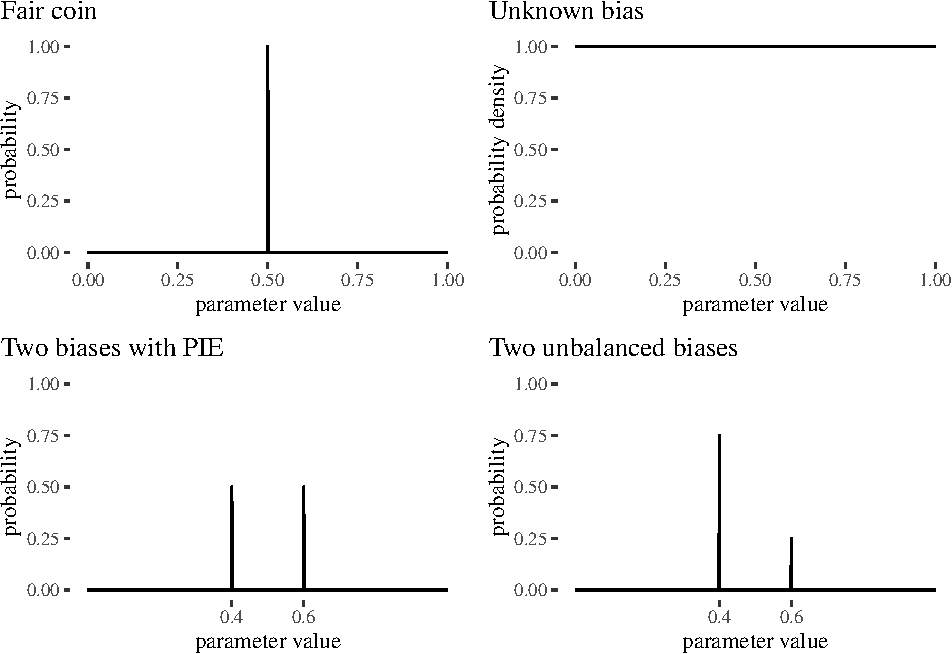
\includegraphics[width=1\linewidth]{imprecision_weight_files/figure-latex/fig:evidenceResponse-1} \end{center}
\caption{Examples of RA's distributions responding to various types of evidence for typical cases brought up in the literature.}



\label{fig:evidenceResponse}
\end{figure}

Summaries of the distributions, such as the expected value, are exactly
that: a simplified and therefore somewhat inadequate representations of
the underlying uncertainty. However, for some purposes---when
simplification is desirable and brings no serious harm---they might be
useful. One summary that comes in handy is the highest density interval
(HDI). It is the narrowest interval containing a specified probability
mass. HDIs are to be contrasted with credible intervals, which span
between \(\nicefrac{\alpha}{2}\) and \(1-\nicefrac{\alpha}{2}\)
quantiles of the probability mass. The key difference is that credible
intervals symmetrically get rid of tails of a distribution, which might
make sense if the distribution is fairly symmetrical, but fails to be
intuitive in other cases.

How to use the higher-order approach in qualitative comparisons? Suppose
the agent's HDIs for probability parameters \(a\) and \(b\) associated
with propositions \(A\) and \(B\) respectively have limits
\(a_l, a_h, b_l, b_h\) (\(a\) low, \(a\) high, \dots) respectively. We
can say that the agent definitely considers \(A\) at least as likely as
\(B\) (\(A\geq B\)) just in case \(a_l\geq b_l\) and \(a_h \geq b_h\),
that \(A>B\) iff \(A\geq B\) but not \(B \geq A\), and that the agent
considers \(A\) plausible just in case \(a_l>t\) for some sensibly high
threshold \(t\). This allows for clear-cut cases, but also for cases in
which the agent is undecided, either about a comparison or about the
plausibility a single proposition. This approach handles Rinard's
GREEN-MYSTERY argument against the supervaluationist approach to
qualitative comparison in \textsf{IP}. Now we are comparing HDIs
instead. For the GREEN urn, the HDI is just \(g=[1,1]\), and since the
distribution is uniform for the MYSTERY urn, its corresponding HDI is
\(m = [0,1]\). In this setting, clearly \(g_l> m_l\) and
\(g_h \geq m_h\), and so \(G\geq M\), but not \(M\geq G\), and therefore
\(G>M\). That is, the agent is more convinced about \(G\) than they are
about \(M\), as desired.

Another difficulty for \textsf{IP} is belief inertia. In this framework,
the problem does not arise, as there is no problem with modeling
learning from observation starting from a uniform prior.

If you just start with a uniform density over \([0,1]\) as your prior,
use binomial probability as likelihood, observing any non-zero number of
heads will exclude 0 and observing any non-zero number of tails will
exclude 1 from the basis of the posterior. Let's see an example with a
grid approximation (\(n=1k\)). For simplicity assume there are only
green and black balls. Our prior is uniform, and then, in subsequent
steps, we observe one green ball, another green ball, and then a black
ball. This is what happens with the posterior as we go (Figure
\ref{fig:intertia2}).

\begin{figure}[H]

\begin{center}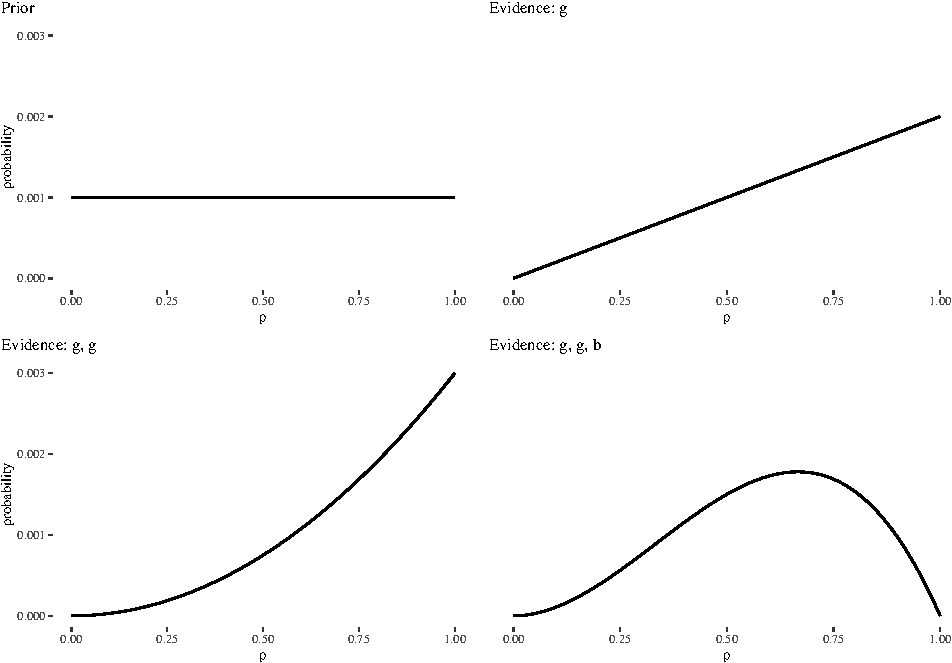
\includegraphics[width=1\linewidth]{imprecision_weight_files/figure-latex/fig:inertia2-1} \end{center}
\caption{As observations of green, green and black come in, extreme parameter values drop out of the picture and the posterior is shaped by the evidence.}
\label{fig:intertia2}
\end{figure}

To see how this approach is also capable of modeling Rinard's example of
inertia, lets start with MaxEnt recommending even priors of the two
chance hypotheses. In Figure 10 we see what usual calculations revise
these priors to, as we obtain new evidence, again, say: green, green,
black. This behaves completely as expected with no inertia in sight.
Note how the observations initially support \(H_1\), but exclude \(H_1\)
in the last stage.

\begin{center}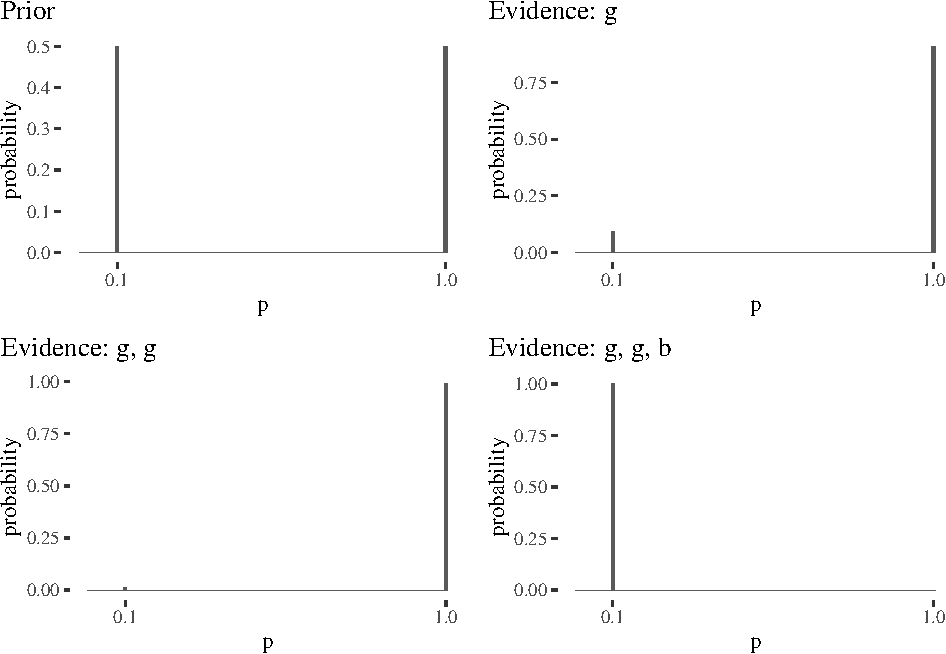
\includegraphics[width=1\linewidth]{imprecision_weight_files/figure-latex/rinardCalculations-1} \end{center}

\begin{figure}[H]

\caption{Learning in Rinard's example of belief inertia.}
\label{fig:rinard2}
\end{figure}

\todo{Talk about other objections here}

\hypertarget{weight-of-a-distribution}{%
\section{Weight of a distribution}\label{weight-of-a-distribution}}

In order to be able to explain our explication of the notion of weight
of evidence, we first need to introduce the information-theoretic
background against which the explication will be developed. Consider a
fairly simple binary case. Suppose you want to navigate from \(A\) to
\(D\), with the uninformed prior, at each junction thinking that each
choice is equally likely to be the right one, your choices are
visualized in Figure \ref{fig:entDAG}.

\begin{figure}[H]

\begin{center}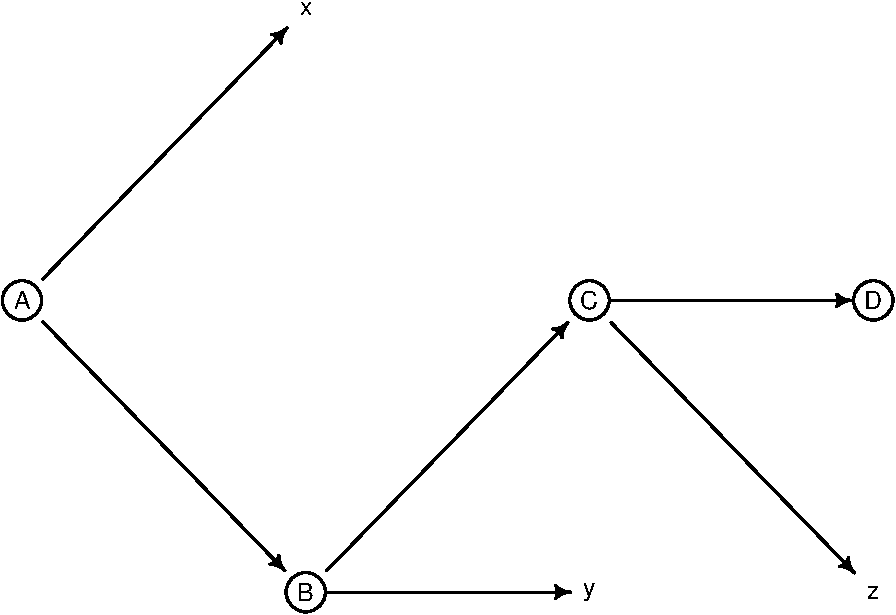
\includegraphics[width=0.7\linewidth]{imprecision_weight_files/figure-latex/label-1} \end{center}
\caption{You want to navigate from $A$ to $D$ with the uninformed prior.}
\label{fig:entDAG}
\end{figure}

The route can be described using three digits. Suppose at each point the
path on the left is marked 1, and the one on the right is marked 0. The
right path is then 011. There are \(m=8\) possible destinations that
could be reached by making decisions at \(\log_2(8)=3\) forks.

How much information are you given if I just tell you to take path 0 at
the first fork? Initially, you thought the probability that it is the
right one was .5. Now you know it is the right one. One natural measure
is \emph{surprise}, \(\nicefrac{1}{.5}=2\): there is a sense in which
you now have twice the information that you had. If to make sure your
measure of information is also additive, you transform surprise
logarithmically, the \emph{Shannon information} is
\(\log_2(\nicefrac{1}{.5})=1\). That is, you receive one \emph{bit} of
information. If you receive the complete instructions, assuming your
probabilities were independent, you receive
\(\log_2(\nicefrac{1}{.5^3})=3\). Thus, intuitively, Shannon's
information tracks the information you received in terms of how many
binary decisions you are now able to make assuming you initially thought
the options were equally likely and independent. Further, notice that
\(\log_2(\frac{1}{a})= - \log_2(a)\) in general, so the official
definition of Shannon information goes: \begin{align*}
h(x) & = - \log_2 \mathsf{\pr{x}}
\end{align*} If the outcomes are equally likely, \(h(x)\) doesn't depend
on the choice of \(x\). However, if the distribution is not uniform,
this will not be the case. A measure of (lack of) information contained
in a whole distribution, is \emph{entropy}, which is the average Shannon
information: \begin{align*}
H(X)  & = \sum \mathsf{P}(x_i) \log_2 \frac{1}{\mathsf{P}(x_i)} =
- \sum \mathsf{P}(x_i) \log_2 \mathsf{P}(x_i)
\end{align*} \noindent Note that entropy is not the measure of
information contained in a distribution. It is rather the opposite: the
expected amount of information you receive once you learn what the value
of \(X\) is. The less informative a distribution is, the more you expect
to learn when you find out the value of \(X\), the higher the entropy.
Also, note that entropy is the function of the measure itself, so
normally it makes sense to talk about the entropy of distributions
rather than variables.

Interestingly, the move to continuous distributions is not
straightforward,\footnote{One might expect that entropy in the continous
  case could be made by binning and taking the limit. For instance,
  suppose we divide \(X\) into bins \(x_i\) of length \(\Delta\), so
  that we discretize \(X\) into \(X^\Delta\). The discrete case
  definition applies: \begin{align*}
  H(X^\Delta) & = \sum \left[\mathsf{P}(X \mbox{ is in the $i$-th bin}) \log_2 \frac{1}{\mathsf{P}(X \mbox{ is in the $i$-th bin})}\right]
  \end{align*} \noindent If you think of the histogram of the
  distribution of \(X^\Delta\) with total area \(A\), each bin has area
  \(a_i\) and height \(p_i\). Suppose we normalize so that \(A =1\),
  then the probability of each bin is \(\mathsf{P}_i = p_i \Delta\) and
  \(p_i\) can be thought of probability density. Then we have:
  \begin{align*}
  H(X^\Delta) & = \sum \mathsf{P}_i \log_2 \frac{1}{\mathsf{P}_i}\\
  & = \sum p_i \Delta \log_2 \frac{1}{p_i \Delta}\\
  & = \sum \left[ p_i \Delta \left(\log_2 \frac{1}{p_i} + \log_2\frac{1}{\Delta}\right)\right]\\
  & = \sum p_i \Delta \log_2 \frac{1}{p_i} +    \underbrace{\sum \underbrace{p_i \Delta}_{\mathsf{P}_i}}_1 \log_2\frac{1}{\Delta} \\
  & = \sum p_i \Delta \log_2 \frac{1}{p_i} +  \log_2\frac{1}{\Delta}
  \end{align*} \noindent Accordingly, when we try to go continuous by
  taking the limit, we get: \begin{align*}
  H(X) & = \left[\int_{-\infty}^\infty p(x) \log_2 \frac{1}{p(x)}\, dx  \right] + \infty
  \end{align*} \noindent This is as it should: the entropy of a
  continuous variable increases with the precision of measurement, so
  infinite precision gives infinite information. For this reason, for
  the continuous case it is usual to drop the rightmost part of the
  equation and talk about \emph{differential entropy}: \begin{align*}
  \mathsf{H}(X) & = \left[\int_{-\infty}^\infty p(x) \log_2 \frac{1}{p(x)}\, dx  \right] 
  \end{align*}}, so in what follows we prefer to stick to entropy
proper. One reason is that we will want to meaningfully compare
information conveyed by discrete distributions to that conveyed by
continuous ones. A convenient way to do so is to abandon the idea that
we should be infinitely precise, fix a certain number of bins (that is a
certain level of precision) and keep it fixed in our comparison. This is
what we will do: effectively, we will be using
\emph{grid approximations} of continuous distributions: we will split
\(X\) into a 1000 bins and use the normalized densities for their
centers to obtain their corresponding probabilities. As long as we do
not change our level of precision (which would inevitably lead to
changes in entropy) in our comparisons, this is not a problem. An
additional advantage is that now we do not have to deal with the
intricacies of explicit analytic calculations for continuous variables
and comparing apples (entropy) with oranges (differential entropy).

Now, let us move forward towards a way to measure differences between
distributions. First, the notion of \emph{cross-entropy}. Suppose events
arise according to a distribution \(\mathsf{P}\) but we predict them
using a distribution \(\mathsf{Q}\). The \emph{cross-entropy} in such a
situation is \begin{align*}
\mathsf{H}(\mathsf{P}, \mathsf{Q}) & = \sum \mathsf{P}_i \log_2(\mathsf{Q}_i)
\end{align*} This value is going to be higher than the entropy of
\(\mathsf{P}\) itself, if \(\mathsf{Q}\) is different from
\(\mathsf{P}\). Now think about the additional entropy introduced by
using \(\mathsf{Q}\) instead of \(\mathsf{P}\) itself, called
\emph{Kullback-Leibler divergence} (KL divergence): \begin{align*}
\mathsf{DKL}(\mathsf{P}, \mathsf{Q}) & = H(\mathsf{P}, \mathsf{Q}) - H(\mathsf{P})\\
&= - \sum \mathsf{P}_i \log_2(\mathsf{Q}_i)  - \left(   - \sum \mathsf{P}_i \log_2 \mathsf{P}_i\right) \\
& = - \sum \mathsf{P}_i\left( \log_2 \mathsf{Q}_i - \log_2\mathsf{P}_i\right)\\
& =  \sum \mathsf{P}_i\left( \log_2 \mathsf{P}_i - \log_2\mathsf{Q}_i\right)\\
& = \sum \mathsf{P}_i \log_2 \left( \frac{\mathsf{P}_i}{\mathsf{Q_i}}\right)
\end{align*} \noindent  That is, KL divergence is the expected
difference in log probabilities. In particular, if
\(\mathsf{P}=\mathsf{Q}\) we get
\(DKL(\mathsf{P},\mathsf{P}) = \sum \mathsf{P}_i (\log_2 \mathsf{P}_i - \log_2 \mathsf{P}_i) = 0\),
which works out as it intuitively should be.\footnote{Note that often in
  the context of Bayesian inference, the natural logarithm function is
  used in the divergence calculations; this only is a shift of scale and
  doesn't make much difference.}

Now, we can introduce the notion of weights as associated with
distributions. In this sense, weights are just transformed distances
from uniform distributions, giving us an information-theoretic measure
of how uneven (or informative) a distribution is. Once we go over this,
we will explain how to implement this approach to evidence. Once we can
measure how uneven the posterior is compared to the prior, we have an
explication of the notion of weight of evidence. It will be, of course,
dependent on the priors---but this we take it to be intended and in line
with the intuitions standing behind the earlier proposals (and if you
prefer to compare posterior with the posterior given the negation of the
evidence, the move is rather straightforward).
\todo{Discuss how deep we want to get into this}

The idea is that the more informative a piece of evidence is, as
compared to the uniform distribution, the more weight it has, on scale 0
to 1: if the drop from uncertainty is complete, the entropy drops to
zero, and we would like the weight to be 1, if the drop is null we would
like to be zero, and if the drop is half, we would like to be .5 (and so
on for other proportions). This can be achieved by the following
definition: \begin{align*}
\mathsf{w(P_i)} & = 1 - \left( \frac{H(\mathsf{P})}{H(\mathsf{uniform})}\right)
\end{align*} \noindent where \(\mathsf{P}\) is the discrete probability
distribution for a given number of bins \(n\), and uniform is the
discrete uniform distribution for the same number of bins.\footnote{In
  some contexts it might make sense to measure improvement with respect
  to a non-uniform prior. In such cases, \(H(\mathsf{uniform})\) is to
  be replaced by \(H(\mathsf{prior})\).} Note that the entropy of a
uniform distribution is pretty straightforward, so we can simplify:
\begin{align*}
H(\mathsf{uniform}) & = \sum_{i=1}^n \nicefrac{1}{n} \log_2 \frac{1}{\nicefrac{1}{n}} \\
& = \log_2(n) \\
\mathsf{w(P_i)} & = 1 - \left( \frac{H(\mathsf{P})}{\log_2(n)}\right)
\end{align*}

Let's first see how this plays out with beta distributions.\footnote{The
  reader might ask: why not to use the Kullback-Leibler divergence from
  the uniform distribution instead? Because this divergence does not
  measure the difference in how informed the distribution is. For
  instance, the divergence between a uniform distribution with a grid of
  \(1k\) and a distribution that gives probability 1 to one chance
  hypotheses and 0 to all others, measured either way, is not going to
  be large, whereas for our purposes the weight should be maximal: we
  just went from complete lack of information to complete certainty.
  This intuition is vindicated when we use \(w\).} The advantage of
looking at them first is that they have a fairly straightforward
interpretation: \(\mathsf{beta(a,b)}\) is the distribution one should
have when tossing a coin with unknown bias, having observed (or
imagining to have observed) \(a\) heads and \(b\) tails, imagining that
seeing one heads and one tails leaves you uninformed. From this
perspective, \(\mathsf{beta(1,1)}\) is the uniform distribution,
\(\mathsf{beta(40,10)}\) is the likelihood corresponding to 40 heads and
10 tails, and so on. To get a feel for what beta distributions look
like, inspect Figure \ref{fig:betas}. Remember we're working with a grid
approximation (\(n=1k\)).

\begin{figure}[H]


\begin{center}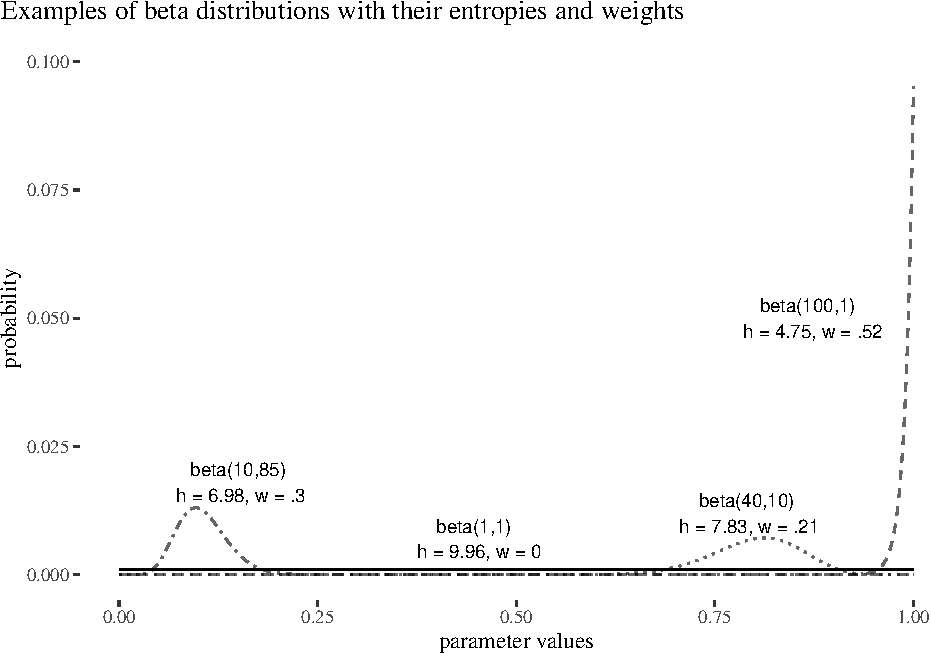
\includegraphics[width=1\linewidth]{imprecision_weight_files/figure-latex/fig:betas3-1} \end{center}
\caption{Examples of beta distributions with entropies and their weights with grid approximation ($n=1000$). Note that distribution weight does not strongly depend on its expected value.}
\label{fig:betas}
\end{figure}

Now let us get back to the example we used to inspect the behavior of
Joyce's proposal. Figure \ref{fig:entropyJoyceExamplePlot} illustrates
dependency on frequency and on priors for sample size \(10\), and
\ref{fig:entropyJoyceExamplePlot100} for sample size 100.

\begin{center}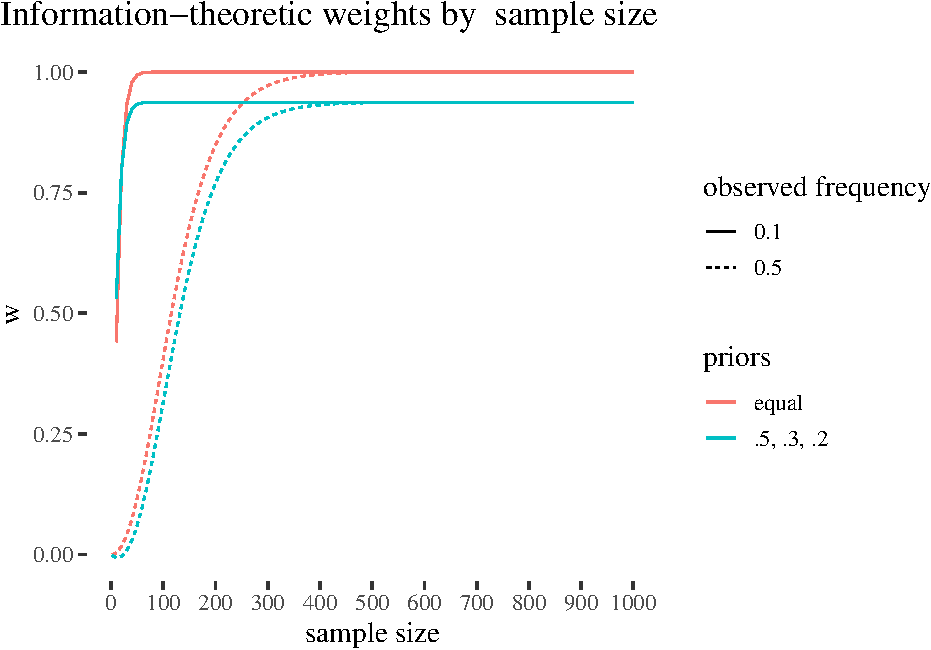
\includegraphics[width=1\linewidth]{imprecision_weight_files/figure-latex/entropyJoyceExample-1} \end{center}

\begin{figure}

\begin{center}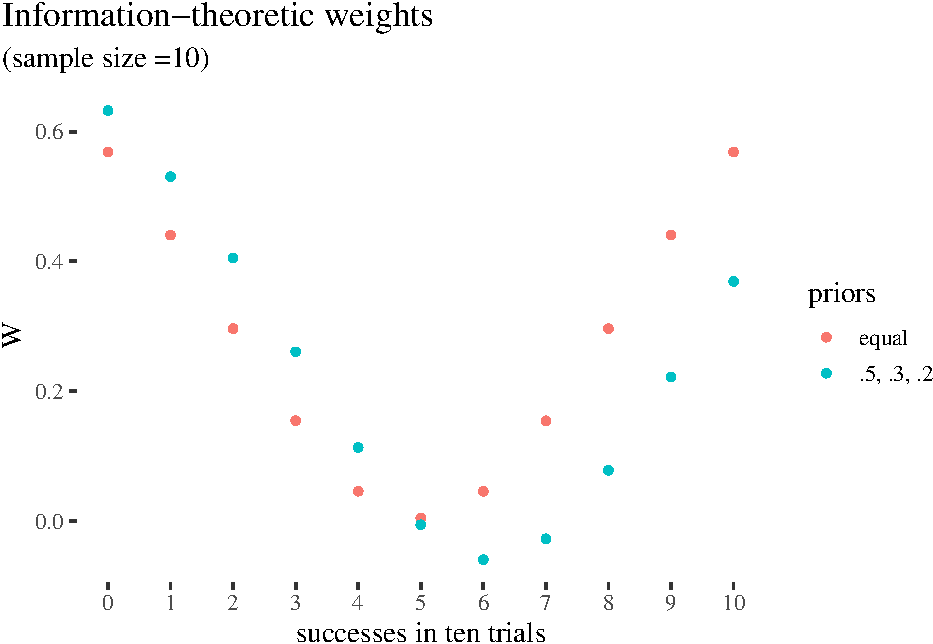
\includegraphics[width=1\linewidth]{imprecision_weight_files/figure-latex/entropyJoyceExamplePlot10-1} \end{center}

\caption{Entropy-based weight for for various observed successes in 10 Bernoulli trials. Three chance chypotheses: $.4, .5, .6$, and two sets of priors: equal and $.5, .3, .2$ respectively.}
\label{fig:entropyJoyceExamplePlot}
\end{figure}

\begin{figure}

\begin{center}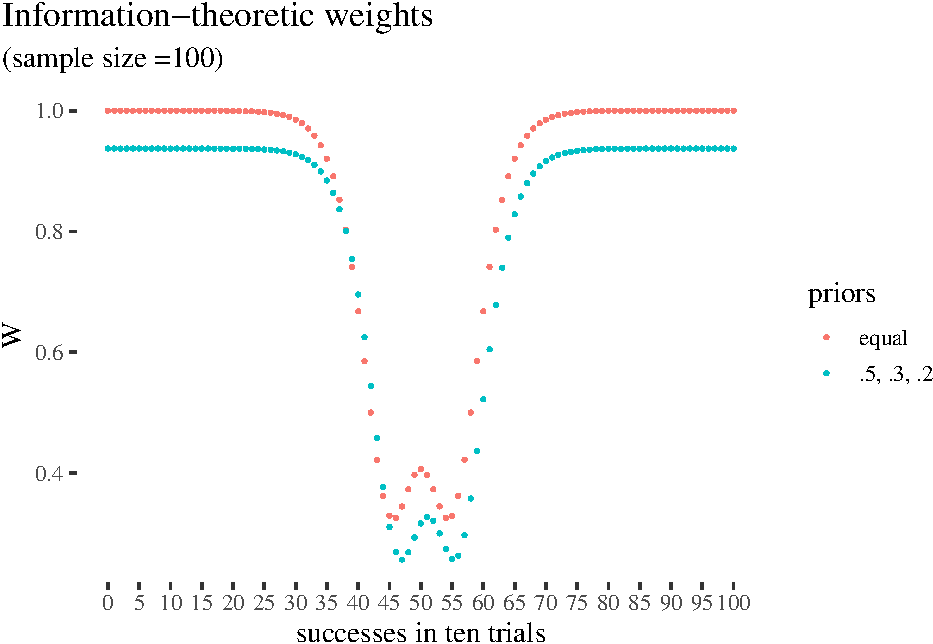
\includegraphics[width=1\linewidth]{imprecision_weight_files/figure-latex/entropyJoyceExamplePlot100-1} \end{center}

\caption{Entropy-based weight for for various observed successes in 100 Bernoulli trials. Three chance chypotheses: $.4, .5, .6$, and two sets of priors: equal and $.5, .3, .2$ respectively.}
\label{fig:entropyJoyceExamplePlot}
\end{figure}

We also should inspect the behavior of \(w\) when the frequency is kept
fixed, but the sample size increases (Figure
\ref{fig:entropyJoyceExampleSampleSize}).

\begin{figure}

\begin{center}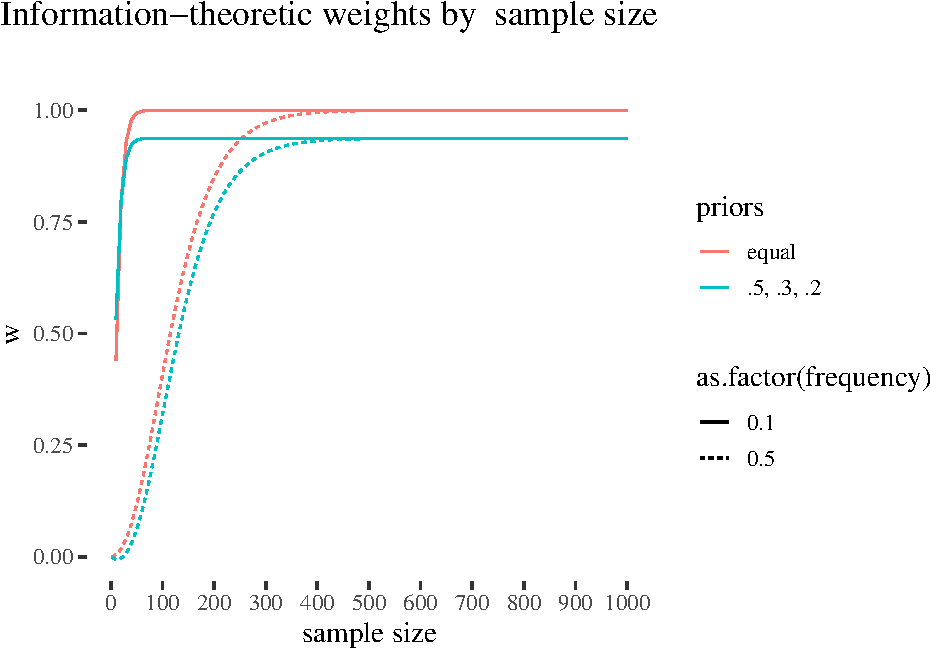
\includegraphics[width=1\linewidth]{imprecision_weight_files/figure-latex/entropyJoyceExampleSampleSize-1} \end{center}

\caption{Entropy-based weight for two observed frequencies for various sample sizes (lines used instead of points for smoothing). Three chance chypotheses: $.4, .5, .6$, and two sets of priors: equal and $.5, .3, .2$ respectively.}
\label{fig:entropyJoyceExampleSampleSize}
\end{figure}

\todo{compare with Joyce, revise comments there and add comments here}

Now, let us generalize and see how the measure behaves with respect to
beta distributions. Two phenomena are as expected. First, the entropy
decreases with the number of observations, and second, it decreases
faster if the proportions are closer to the extremes. This is mirrored
by the corresponding weights (Figure \ref{fig:weights}).

\begin{figure}[H]

\begin{center}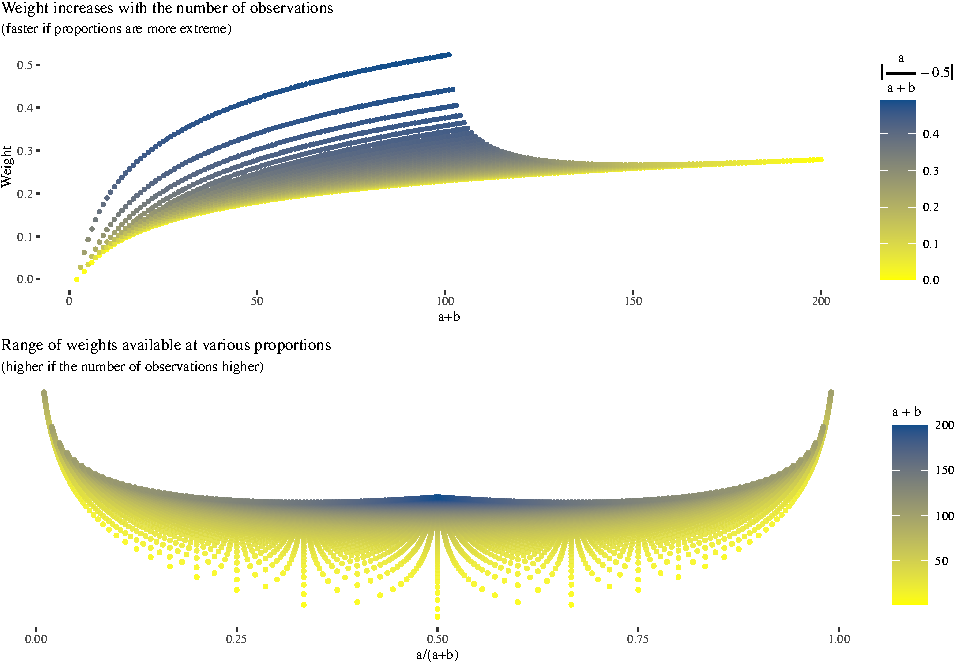
\includegraphics[width=1\linewidth]{imprecision_weight_files/figure-latex/fig:weights-1} \end{center}
\caption{Weights of beta likelihoods for $a,b$ ranging from $0$ to $100$, versus the number of observations   and versus absolute distance of the proportion from .5.}
\label{fig:weights}
\end{figure}

Moreover, the framework is capable of sensible comparison of weights for
distributions of various shapes, including those involving all weights
focused on a particular point (strictly speaking, a single bin in the
grid approximation). Here are some examples of shapes worth looking at
(Figure \ref{fig:weightsWeird}).

\begin{figure}[H]

\begin{center}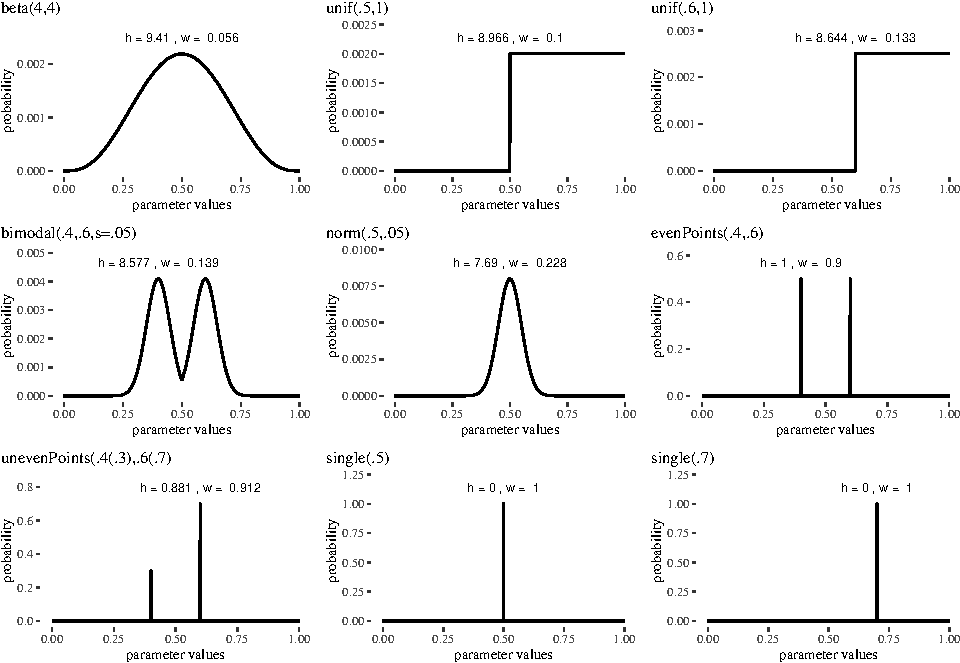
\includegraphics[width=1\linewidth]{imprecision_weight_files/figure-latex/fig:weightsWeird-1} \end{center}
\caption{Examples of various distributions with their entropies and weights, ordered by weights. (1) beta(4,4), (2) uniform starting from .5 to 1, (3), uniform strating from .6 to 1, (4) two normal distributions centered around .4 and .6 with standard deviation .05, glued at .5. (5) normal centered around .5 with the same standard deviation, (6) one that assigns .5 to each of .4  and .6, (7) One that assigns .3 to .4 and .7 to .6., (8) one that assigns all weight to .5, and (9) one that assigns all weight to .7.}

\label{fig:weightsWeird}
\end{figure}

Note that the ordering of weights is as expected. Partial uniform
likelihoods which exclude at least half of parameter values have more
weight than a weak beta, and the weight increases as the non-zero
interval of the partial uniform distribution decreases. A bimodal normal
distribution ``glued'' from two normal distributions carries less weight
than a unimodal normal distribution with the same standard deviation
centered around the mean of the two modes, all these are way below point
estimates. If multiple points have non-zero probability, the weight
depends on how uneven the distribution is, whereas if full weight is
given to a single point, the value of the parameter is known, the weight
is maximal (=1) and does not depend on what the parameter is.

\todo{Comment about the desiderata listed in the beginning}

\hypertarget{weight-of-evidence}{%
\section{Weight of evidence}\label{weight-of-evidence}}

So far we have discussed the weight of a distribution, meant to measure
how informed an agent is about an issue. If the agent starts with a
uniform prior, this is a good enough approximation of how informed the
evidence made them. But in general, how much more information is
obtained is context-dependent. We want a prior-relative notion of
weight, following the intuition that weight consideration should guide
our information gathering also in making us stop collecting further
evidence in light of what we already know. But for weight of evidence to
have this feature, it has to depend on what we already know.

So here is a general recipe. In a given context, consider your
distribution for the target hypothesis \(H\) given what you already
know. Then update on the evidence. This might increase the weight for
\(H\), if the evidence confirms your conviction, or decrease it, if it
goes against what the previous evidence tells you. Take the difference
between the prior weight and the posterior weight (\(\Delta w\)) as your
measure of the weight of evidence in that context. If you prefer to
think that weight of evidence should be always positive, you might
prefer the absolute value thereof. We, however, prefer to keep track of
whether the evidence makes you more or less confused. The calculation
goes along the following schema:

\begin{enumerate}
\item Start with a prior distribution over the parameter space of interest, and with distributions expressing the agent's uncertainty about other probabilities involved in the calculation of the posterior.
\item Sample from these distributions.
\item For each sample, treat it as a selection of precise probabilities, apply Bayes' theorem to calculate the posterior.
\item The set of the results is the sampling distribution expressing your posterior uncertainty.
\end{enumerate}

For instance, suppose that you learn that if a child has been the victim
of abuse, your prior given everything else you know is
\(\mathsf{beta}(2,4)\) with median at .31, the conditional probability
that they will have the habit of rocking if they have been a victim has
a point estimate of .3. How strong is the evidence when you observe a
given child rocks? Well, this depends on how probable rocking is given
that the child has not been abused. This is the lesson that we learned
in the chapter on likelihood ratio. So first, consider two scenarios, in
which this conditional probability also receives a point estimate.
First, \(.2\), then \(.05\). Finally, with conditional probabilities
also being uncertain, say \(\pr{E \vert A}\) coming from normal
distribution with \(\mu = .3, \sigma = .1\), truncated to \((0,1)\), and
\(\pr{E\vert \n A}\) coming from normal distribution with \(\mu = .05\)
and \(\sigma = .05\), corresponding to the idea that the sample of
non-abused children is much larger, and the uncertainty about rocking
about non-abused children is lower. The corresponding shifts from the
prior to the posteriors (with sample size \(1e7\)) are pictured in
Figure \ref{fig:abuse1}.

\begin{figure}[H]

\begin{center}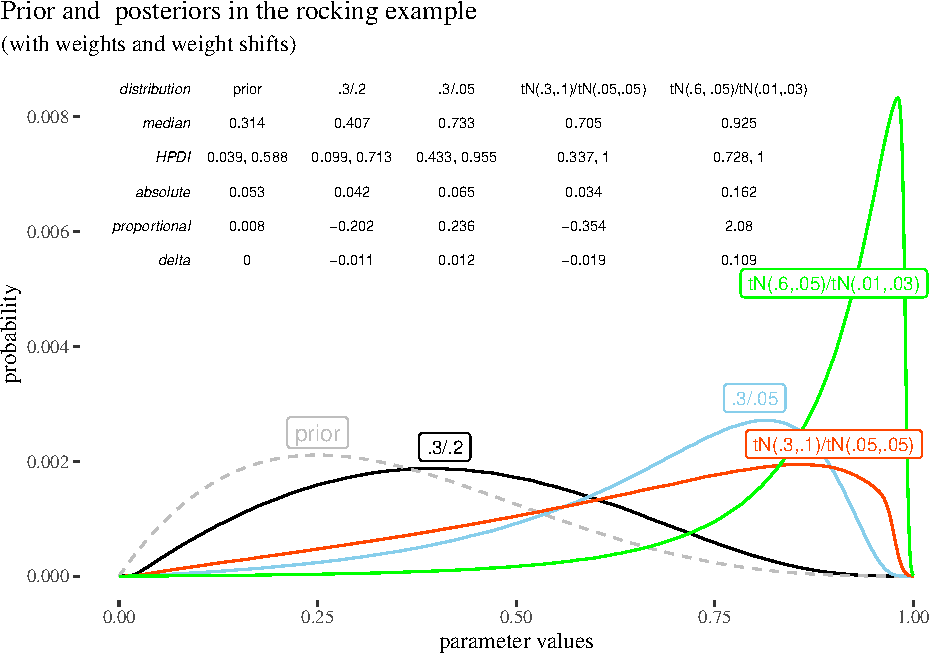
\includegraphics[width=1\linewidth]{imprecision_weight_files/figure-latex/fig:abuse4c-1} \end{center}
\caption{Shifts from prior $\mathsf{beta}(2,4)$ to the posteriors, given various conditional probabilities.}
\label{fig:abuse1}
\end{figure}

\todo{tried to find stats on rocking in abused vs non-abused children, failed}

\hypertarget{completeness-tends-to-improve-weight}{%
\section{Completeness tends to improve
weight}\label{completeness-tends-to-improve-weight}}

\hypertarget{weight-tends-to-improve-accuracy}{%
\section{Weight tends to improve
accuracy}\label{weight-tends-to-improve-accuracy}}

Here is a question asked by {[}COHEN 1986 TWELVE p.~276{]}: is it worth
while knowing the weight of an argument without knowing its probability?
In our terminology, questions inspired by Cohen's are: what's the point
of weight considerations if we already have the distributions? Can
weights be put to use if we do not have the distributions?

First, we need to explain how accuracy is to be measured in this
framework. We already know what accuracy measures are on the market for
single probability measures, and we know that proper scoring rules for
representors are not forthcoming. What is the situation with the
higher-order approach that we propose? The idea is conceptually
straightforward. We take the inaccuracy of a (discretized) distribution
\(p\) from a given true chance/single rational probability hypothesis by
taking the Kulback-Leibler divergence from the indicator distribution of
this hypothesis to \(p\).

More formally, take probability distribution \(p\) over a
grid-approximated parameter space, assigning probabilities
\(p_1, \dots, p_n\) to \(\theta_1, \dots, \theta_n\) respectively. It is
to be evaluated in terms of inaccuracy from the perspective of a given
``true'\,' value \(\theta_k\).\footnote{Two caveats: if you prefer to
  think of evaluation with respect to truth and falsehood only, the only
  ``true values'' to be used are 0 and 1. If on the other hand, you
  think the true distribution does not have to be an indicator
  distribution assigning value 1 to exactly one hypothesis, evaluate the
  Kullback-Leibler distance from this more complex distribution. Such
  decisions can be accommodated in our framework.} The inaccuracy of
\(p\) if \(\theta_k\) is the ``true'' value, is the divergence between
\(IndI^k\) and \(p\). \footnote{Another option is continuous ranked
  probability score (CRPS) of a distribution \(p\) with respect to a
  possible world \(w\): \begin{align*}
  I(p,w) &= \int_{-\infty}^\infty \vert \mathsf{P}(x) - \mathbf{ 1 }(x\geq V(w))\vert ^2 \, dx
  \end{align*} \noindent where \(\mathsf{P}\) is the cumulative
  probability corresponding to a given density, and \begin{align*}
  \mathbf{ 1 }(x \geq V(w)) & = \begin{cases} 1 & \text{ if } x \geq V(w)\\
  0 & \text{ o$\,$/w. }
  \end{cases}
  \end{align*} \noindent  The intuition here is that the measure takes
  the Cramer-Von-Mises measure of distance between densities, defined in
  terms of the area under the squared euclidean distances between the
  corresponding cumulative density functions: \begin{align*}
  \mathcal{C}(p,q) & = \int_{0}^{1} \vert P(x) - Q(x)\vert^2 \, dx
  \end{align*} \noindent and uses it to measure distance to an
  epistemically omniscient chance hypothesis, which either puts full
  weight on 0, if a given proposition is false, or on 1, otherwise. We
  do not use this measure, as it is more complicated than necessary,
  uses square distances instead of information-theoretic notions which
  makes it somewhat more arbitary (and we have seen how squaring played
  out in our discussion of Joyce's proposal), and because it has
  unintuitive features when it comes no multi-modal distributions (SEE
  AUTHOR'S PAPER FOR DETAILS)}

\begin{align*}
\mathcal{I}_{\mathsf{DKL}}^2(p, \theta_k) & = \mathsf{DKL}(Ind^k,p) \\
& = \sum_{i=1}^n Ind^k_i \left( \log_2 Ind^k_i - \log_2 p_i \right)
\end{align*}

It has been proven {[}CITE AUTHOR'S PAPER{]} that the resulting measure
of inaccuracy is a proper scoring rule. Another interesting feature of
the framework is that the point made by Schoenfield against \textsf{IP}
does not apply here: there are cases in which accuracy considerations
recommend an imprecise stance (that is, a multi-modal) distribution over
a precise one. Here is a quick example. Suppose the opponent will
produce two coins, one with the distribution of Heads either normal
around \(.3\), and one normal around \(.5\), both with the standard
deviation of \(.05\), randomly pick one of these coins and then toss it.
The agent knows the setup. Consider the following three (out of many)
possible stances that the agent could take:

\begin{figure}[H]

\begin{center}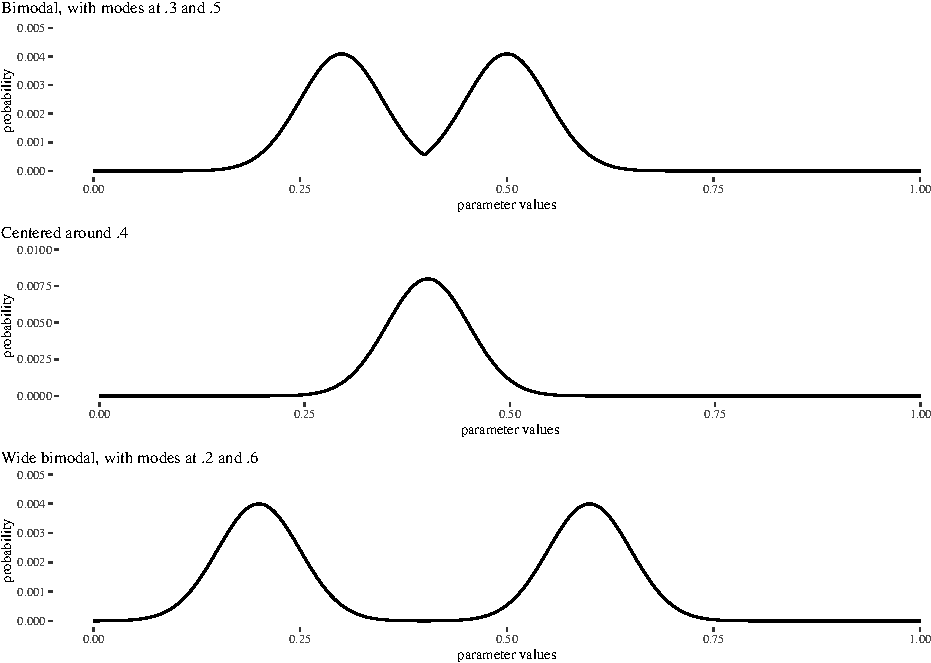
\includegraphics[width=1\linewidth]{imprecision_weight_files/figure-latex/figEMC-1} \end{center}
\caption{Three (out of many) candidate distributions for a Schoenfield-inspired example. All distributions are built from normal  distributions with standard deviation $.5$, the bimodal ones are "glued" in the middle.}
\label{fig:EMC}
\end{figure}

For the three distributions we're discussing in this chapter, the
inaccuracies calculated using CRPS and KL divergence with respect to
various potential true probability distributions look as in Figure
\ref{fig:inaccuracies2}.

\begin{figure}[H]

\begin{center}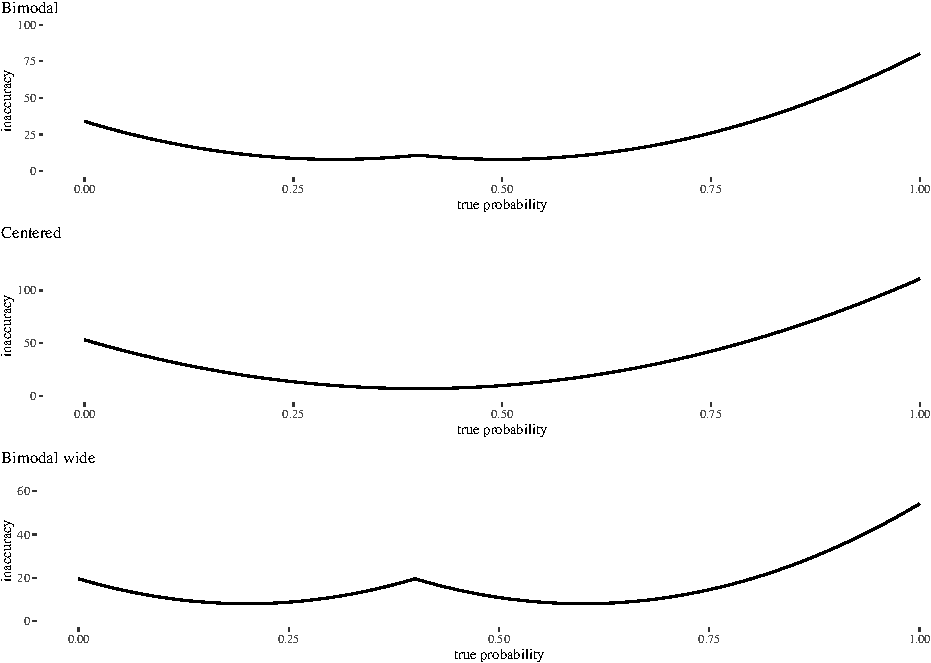
\includegraphics[width=1\linewidth]{imprecision_weight_files/figure-latex/fig:inaccuracies2-1} \end{center}
\caption{KL divergence inaccuracies vs (omniscient functions corresponding to) $n$ true probability hypotheses for the three distributions discussed in this section.}
\label{fig:inaccuracies2}
\end{figure}

\hypertarget{literature-to-discuss}{%
\section{Literature to discuss}\label{literature-to-discuss}}

Kasser, 2016, Two Conceptions of Weight of Evidence in Peirce's
Illustrations of the Logic of Science {[}COVERED{]}

Feduzi, 2010, On Keynes's conception of the weight of evidence COVERED

Cohen 1986, Twelve Questions about Keynes's Concept of Weight
{[}COVERED{]}

Pedden, William 2018, Imprecise probability and the measurement of
Keynes' weight of arguments {[}GET BACK TO INERTIA, DILUTION ETC.{]}

Levi 2011, the weight of argument {[}DOWNLOADED{]}

Skyrms 1977 resiliency, propensities {[}DOWNLOADED{]}

Skyrms causal necessity, chapter on resilience {[}DOWNLOAD{]}

Synthese 186 (2) 2012, volume on Keynesian weight {[}CHECKED, NOT MUCH
ON WEIGHT ACTUALLY, NO NEED TO READ{]}

Good, weight of evidence, survey

Good, PROBABILITY AND THE WEIGHING OF EVIDENCE

David Hamer, Probability, anti-resilience, and the weight of expectation
{[}READ{]}

William Peden, Imprecise Probability and the Measurement of Keynes's
``Weight of Arguments''

Runde, Keynesian Uncertainty and the weight of arguments
{[}DOWNLOADED{]}

Weatherson, 2002, Keynes, uncertainty and interest rates
{[}DOWNLOADED{]}

Jeffrey M. Keisler, Value of information analysis: the state of
application

Edward C. F. Wilson, A Practical Guide to Value of Information Analysis

Joyce JM (2005) How probabilities reflect evidence.

Kyburg. Probability and the Logic of Rational Belief. Wesleyan
University Press, Middletown Connecticut, 1961

H. E. Kyburg and C. M. Teng. Uncertain Inference. Cambridge University
Press, Cam- bridge, 2001.

\hypertarget{refs}{}
\begin{CSLReferences}{1}{0}
\leavevmode\vadjust pre{\hypertarget{ref-bradley2012uncertaintyPhD}{}}%
Bradley, S. (2012). \emph{Scientific uncertainty and DecisionMaking}
(PhD thesis). London School of Economics; Political Science.

\leavevmode\vadjust pre{\hypertarget{ref-bradley2019imprecise}{}}%
Bradley, S. (2019). {Imprecise Probabilities}. In E. N. Zalta (Ed.),
\emph{The {Stanford} encyclopedia of philosophy} ({S}pring 2019).
\url{https://plato.stanford.edu/archives/spr2019/entries/imprecise-probabilities/};
Metaphysics Research Lab, Stanford University.

\leavevmode\vadjust pre{\hypertarget{ref-CampbellMoore2020accuracy}{}}%
Campbell-Moore, C. (2020). \emph{Accuracy and imprecise probabilities}.

\leavevmode\vadjust pre{\hypertarget{ref-Carr2020impreciseEvidence}{}}%
Carr, J. R. (2020). Imprecise evidence without imprecise credences.
\emph{Philosophical Studies}, \emph{177}(9), 2735--2758.
\url{https://doi.org/10.1007/s11098-019-01336-7}

\leavevmode\vadjust pre{\hypertarget{ref-Christensen2009disagreement}{}}%
Christensen, D. (2009). Disagreement as evidence: The epistemology of
controversy. \emph{Philosophy Compass}, \emph{4}(5), 756--767.
\url{https://doi.org/10.1111/j.1747-9991.2009.00237.x}

\leavevmode\vadjust pre{\hypertarget{ref-Dietrich2016pooling}{}}%
Dietrich, F., \& List, C. (2016). Probabilistic opinion pooling. In A.
Hajek \& C. Hitchcock (Eds.), \emph{Oxford handbook of philosophy and
probability}. Oxford: Oxford University Press.

\leavevmode\vadjust pre{\hypertarget{ref-elga2010subjective}{}}%
Elga, A. (2010). \emph{Subjective probabilities should be sharp}.

\leavevmode\vadjust pre{\hypertarget{ref-Elkin2018resolving}{}}%
Elkin, L., \& Wheeler, G. (2018). Resolving peer disagreements through
imprecise probabilities. \emph{Noûs}, \emph{52}(2), 260--278.
\url{https://doi.org/10.1111/nous.12143}

\leavevmode\vadjust pre{\hypertarget{ref-VanFraassen2006vague}{}}%
Fraassen, B. C. V. (2006). Vague expectation value loss.
\emph{Philosophical Studies}, \emph{127}(3), 483--491.
\url{https://doi.org/10.1007/s11098-004-7821-2}

\leavevmode\vadjust pre{\hypertarget{ref-Gardenfors1982unreliable}{}}%
Gärdenfors, P., \& Sahlin, N.-E. (1982). Unreliable probabilities, risk
taking, and decision making. \emph{Synthese}, \emph{53}(3), 361--386.
\url{https://doi.org/10.1007/bf00486156}

\leavevmode\vadjust pre{\hypertarget{ref-joyce2005probabilities}{}}%
Joyce, J. M. (2005). How probabilities reflect evidence.
\emph{Philosophical Perspectives}, \emph{19}(1), 153--178.

\leavevmode\vadjust pre{\hypertarget{ref-Kaplan1968decision}{}}%
Kaplan, J. (1968). Decision theory and the fact-finding process.
\emph{Stanford Law Review}, \emph{20}(6), 1065--1092.

\leavevmode\vadjust pre{\hypertarget{ref-Kaplan1996decision}{}}%
Kaplan, M. (1996). \emph{Decision theory as philosophy}. Cambridge
University Press.

\leavevmode\vadjust pre{\hypertarget{ref-keynes1921treatise}{}}%
Keynes, J. M. (1921). \emph{A treatise on probability, 1921}. London:
Macmillan.

\leavevmode\vadjust pre{\hypertarget{ref-Lee2017impreciseEpistemology}{}}%
Lee, E. (2017). \emph{Imprecise probability in epistemology} (PhD
thesis). Ludwig-Maximilians-Universit{ä}t;
Ludwig-Maximilians-Universität München.

\leavevmode\vadjust pre{\hypertarget{ref-Levi1974ideterminate}{}}%
Levi, I. (1974). On indeterminate probabilities. \emph{The Journal of
Philosophy}, \emph{71}(13), 391. \url{https://doi.org/10.2307/2025161}

\leavevmode\vadjust pre{\hypertarget{ref-Levi1980enterprise}{}}%
Levi, I. (1980). \emph{The enterprise of knowledge: An essay on
knowledge, credal probability, and chance}. MIT Press.

\leavevmode\vadjust pre{\hypertarget{ref-Mayo-Wilson2016scoring}{}}%
Mayo-Wilson, C., \& Wheeler, G. (2016). Scoring imprecise credences: A
mildly immodest proposal. \emph{Philosophy and Phenomenological
Research}, \emph{92}(1), 55--78.
\url{https://doi.org/10.1111/phpr.12256}

\leavevmode\vadjust pre{\hypertarget{ref-Rinard2013against}{}}%
Rinard, S. (2013). Against radical credal imprecision. \emph{Thought: A
Journal of Philosophy}, \emph{2}(1), 157--165.
\url{https://doi.org/10.1002/tht3.84}

\leavevmode\vadjust pre{\hypertarget{ref-Schoenfield2017accuracy}{}}%
Schoenfield, M. (2017). The accuracy and rationality of imprecise
credences. \emph{Noûs}, \emph{51}(4), 667--685.
\url{https://doi.org/10.1111/nous.12105}

\leavevmode\vadjust pre{\hypertarget{ref-seidenfeld2012forecasting}{}}%
Seidenfeld, T., Schervish, M., \& Kadane, J. (2012). Forecasting with
imprecise probabilities. \emph{International Journal of Approximate
Reasoning}, \emph{53}, 1248--1261.
\url{https://doi.org/10.1016/j.ijar.2012.06.018}

\leavevmode\vadjust pre{\hypertarget{ref-Stewart2018pooling}{}}%
Stewart, R. T., \& Quintana, I. O. (2018). Learning and pooling, pooling
and learning. \emph{Erkenntnis}, \emph{83}(3), 1--21.
\url{https://doi.org/10.1007/s10670-017-9894-2}

\leavevmode\vadjust pre{\hypertarget{ref-Sturgeon2008grain}{}}%
Sturgeon, S. (2008). Reason and the grain of belief. \emph{No{û}s},
\emph{42}(1), 139--165. Retrieved from
\url{http://www.jstor.org/stable/25177157}

\leavevmode\vadjust pre{\hypertarget{ref-walley1991statistical}{}}%
Walley, P. (1991). \emph{Statistical reasoning with imprecise
probabilities}. Chapman; Hall London.

\end{CSLReferences}

\end{document}
